\documentclass[11pt]{amsart}

%\usepackage[english]{babel}
%\usepackage[frenchb]{babel}

\usepackage[utf8]{inputenc}
\usepackage[francais,frenchb]{babel}
\usepackage[T1]{fontenc}


%\usepackage{showkeys}
\usepackage{amsmath,dsfont}
\usepackage{amssymb}
\usepackage{cite}
\usepackage{hyperref}

\usepackage{lineno}

\usepackage{microtype}

\DisableLigatures[f]{encoding = *, family = * }
\usepackage{algorithmic}

\topmargin 0.0cm
\oddsidemargin 0.5cm
\evensidemargin 0.5cm
\textwidth 16cm 
\textheight 21cm

\usepackage[labelfont=bf,labelsep=period,justification=raggedright]{caption}

\makeatletter
\renewcommand{\@biblabel}[1]{\quad#1.}
\makeatother


%%%%%  Personalisation de la classe amsart, pour le francais
%%%%%   cf. http://ctan.mines-albi.fr/macros/latex/required/amslatex/amscls/doc/amsclass.pdf
\makeatletter
\def\@@and{et}  %%%%%  <---- pour redefinir le mot "and" devant le dernier auteur dans la liste des auteurs. A placer dans un \makeatletter
\def\curraddrname{{\itshape Adresse}}  %%%%%  <---- pour redefinir le mot "Current address"
\def\emailaddrname{{\itshape Courriel}}  %%%%%  <---- pour redefinir le mot "E-mail address"
\makeatother

\pagestyle{myheadings}

%%% pour debug
%%% \date{\today\\ \shortauthors \\ \authors  \\  \shorttitle \\  \addresses \\  }


%%%%%%%%%%%%%%%%%%%%%%%%%%%%%%%%%%

%\usepackage{datetime}
\usepackage{dsfont}
\usepackage{graphicx}
\usepackage{subfig}


\usepackage{mathtools} %%% pour  \perscript
\usepackage{enumitem} %%% option pour changer les puces des enumerate

\usepackage{pict2e} %% pour avoir de beaux ovales
\usepackage{placeins} %% pour avoir \FloatBarrier
\usepackage{calc}
\usepackage{fp}%% pour les operations arithmetiques
\usepackage{tabularx}
\usepackage[table]{xcolor} %%% Attention, a charger AVANT Tikz
\usepackage{colortbl}%%pour colorer les cellules d un tableau (\rowcolor)
\usepackage{multirow}
\usepackage{xspace}

\usepackage{tablefootnote}

\usepackage{tikz}
\usetikzlibrary{spy}

%\let\oldtabular=\tabular
%\def\tabular{\small\oldtabular}


%%%%%%%%%%%%%--PREAMBLE--%%%%%%%%%%%%%%%%%%
\numberwithin{equation}{section}

\graphicspath{{../img_publi_GIST/}{../img/}}

\newcommand{\etal}{{\it et al.}}
\newcommand{\ie}{i.e.\/}

\newcommand{\CFL}{{\mathrm{CFL}}}
\newcommand{\Id}{{\mathds 1}}

\newcommand{\W}{{\bf W}}

\newcommand{\Frm}{{\rm F}}
\newcommand{\Grm}{{\rm G}}
\newcommand{\Hrm}{{\rm H}}
\newcommand{\crm}{{\rm c}}

\newcommand{\treat}{\mathcal{T}}
%\newcommand{\TI}{{\rm T_1}}
%\newcommand{\TS}{{\rm T_2}}
\newcommand{\TI}{{\mathcal T_1}}
\newcommand{\TS}{{\mathcal T_2}}
\newcommand{\Tini}[1]{\rm{T}_{ini}^#1}
\newcommand{\Tend}[1]{\rm{T}_{end}^#1}
%\newcommand{\chiI}{\chi_{\TI}}
%\newcommand{\chiS}{\chi_{\TS}}
%\newcommand{\chii}{\chi_{\treat_i}}
\newcommand{\chii}{\chi_{\rm i}}
\newcommand{\chiI}{\chi_1}
\newcommand{\chiS}{\chi_2}
\newcommand{\dive}{\nabla\cdot}

\newcommand{\Amin}{\mathcal{A}_{\rm min}}

\newcommand{\TPFS}{{\rm T_{PFS}}}
\newcommand{\Td}{{\rm T_{double}}}

%\newcommand{\muI}{\mu_{\TI}}
%\newcommand{\muS}{\mu_{\TS}}
%\newcommand{\nuS}{\nu_{\TS}}
\newcommand{\muI}{\mu_1}
\newcommand{\muS}{\mu_2}
\newcommand{\nuS}{\nu_2}
\newcommand{\muN}{\delta}

\newcommand{\RR}{{\mathbb{R}}}

\newcommand{\nn}{{\bf n}}
\newcommand{\GG}{{\bf G}}


\newcommand{\ang}{{\mathfrak{a}}}
\newcommand{\ex}{{\bf e}_x}
\newcommand{\ey}{{\bf e}_y}

\newcommand{\er}{{\bf e}_r}
\newcommand{\et}{{\bf e}_{\theta}}

\newcommand{\trans}[1]{\prescript{\mathit{t\!}}{}{#1}}
\newcommand{\gammapp}{\gamma_{pp}}
\newcommand{\gammapd}{\gamma_{pd}}
\newcommand{\gammasd}{\gamma_{sd}}
\newcommand{\Ms}{M_{th}}
\newcommand{\vit}{\mathbf{v}}
\newcommand{\vecx}{\mathbf{x}}
\newcommand{\vecy}{\mathbf{y}}
\newcommand{\Tfini}{{T_f}_{ini}}
\newcommand{\Tgini}{{T_g}_{ini}}
\newcommand{\Tfend}{{T_f}_{end}}
\newcommand{\Tgend}{{T_g}_{end}}
\newcommand{\twinweno}{twin-WENO5}
\newcommand{\Twinweno}{Twin-WENO5}
\newcommand{\ctscan}{CT-scan}
\newcommand{\cf}{\textit{cf.}~}


%\DeclareRobustCommand{\Nber}{Patient~A\@\xspace}
%\DeclareRobustCommand{\Chen}{Patient~B\@\xspace}
\newcommand{\Nber}{Patient~A\xspace}
\newcommand{\Chen}{Patient~B\xspace}

\newcommand{\rect}[4]{
\multiput(#1,#2)(0,#4){2}{\line(1,0){#3}}
\multiput(#1,#2)(#3,0){2}{\line(0,1){#4}}
}

%%%%%%%%%%%%%%%--BODY--%%%%%%%%%%%%%%%%%%
\begin{document}
\title[Modélisation spatiale de résistances aux traitements cancéreux]{Modélisation spatiale de résistance aux traitements cancéreux~: cas des métastases hépatiques de GIST}

\thanks{$1$:~Bordeaux INP, IMB, UMR 5251, F-33400,Talence, France}

\thanks{$2$:~Univ. Bordeaux, IMB, UMR 5251, F-33400, Talence, France}
\thanks{$3$:~INRIA Bordeaux-Sud-Ouest, F-33400,Talence, France}
\thanks{$4$:~Group of Applied Mathematics (GMA) and Group of Tumor
  Angiogenesis (GIANT), Basic Sciences Department, Faculty of
  Sciences, Universidad del B\'\i o-B\'\i o, Campus Fernando May, Chill\'an, Chile}
\thanks{$5$:~Centre for Biotechnology and Bioengineering, University
  of Chile, Beauchef 850, Santiago, Chile}
\thanks{$6$:~CNRS, IMB, UMR 5251, F-33400, Talence, France}
\thanks{$7$:~Service d'imagerie diagnostique et interventionnelle de l'adulte, H\^opital Pellegrin, CHU de Bordeaux, Bordeaux, France}

\author[G. Lefebvre]{Guillaume Lefebvre$^{1,2,3}$}
\email[G. Lefebvre]{guillaume.lefebvre@math.u-bordeaux.fr }

\author[F. Cornelis]{Fran\c cois Cornelis$^{2,7}$}
\email[F.Cornelis]{francois.cornelis@chu-bordeaux.fr}

\author[P. Cumsille]{Patricio Cumsille$^{4,5}$}
\email[P.Cumsille]{pcumsill@gmail.com}

\author[T. Colin]{Thierry Colin$^{1,2,3}$}
\email[T.Colin]{colin@math.u-bordeaux.fr}


\author[C. Poignard]{Clair Poignard$^{3,6}$}
\email[C. Poignard]{clair.poignard@inria.fr}

\author[O. Saut]{Olivier Saut$^{6,3}$}
\email[O. Saut]{Olivier.Saut@math.u-bordeaux.fr}

\maketitle


\begin{abstract}
Ce travail est consacré à la modélisation de métastases hépatiques en provenance de tumeur du stroma gastro-intestinal (GIST), à leur croissance et leurs résistances aux thérapies. On s'intéressera plus précisément aux résistances, observées cliniquement, aux deux traitements standards basés sur des inhibiteurs de tyrosine kinase (imatinib et sunitinib). 
Partant d'observations sur les images médicales (scanners), nous construisons un modèle spatial qui consiste en un système d'équations aux dérivées partielles non linéaire. Après calibration de ses paramètres avec les données cliniques, le modèle reproduit, qualitativement et quantitativement, l'évolution spatiale de la tumeur d'un patient spécifique. D'importants résultats sur la croissance, comme l'apparition de l'hétérogénéité spatiale ou les rechutes, peuvent être expliqués par notre modèle. 
Ensuite, nous investiguons sur la possibilité d'optimiser le traitement numériquement, en terme de temps de survie sans aggravation et en terme de taille minimale atteinte par la tumeur en faisant varier la dose du premier traitement. Selon notre modèle, le temps de survie sans aggravation  atteint un plateau en fonction de la dose. Nous démontrons également numériquement, que la structure spatiale de la tumeur peut fournir plus d'informations sur l'activité des cellules cancéreuses que le critère standard RECIST qui consiste uniquement en la mesure du diamètre de la tumeur. 
Nous discuterons finalement du caractère non prédictif de notre modèle en utilisant seulement des scanners, dans le sens où le comportement de la lésion dans les premiers mois, n'est pas suffisant pour prédire la réponse au traitement. Des données histologiques, comme des biopsies ou de l'imagerie fonctionnelle par exemple, seront intégrées dans de futurs travaux pour palier à ces inconvénients.
\end{abstract}
 \section{Introduction}
Les tumeurs du stroma gastro-intestinal (GISTs) sont les plus communes de toutes les tumeurs 
mésenchymateuses du système gastro-intestinal avec une incidence de 9 à 14 cas par million de personnes par an (\cf \cite{Nilsson2005}). 
Dans 25\% des cas (\cf \cite{dematteo2000}), ce type 
de cancer migre au foie. 


Bien que les GISTs résistent à la plupart des chimiothérapies anticancéreuses conventionnelles, 
%Even though GISTs resist to most of conventional cancer chemotherapies, 
la découverte de mutations actives du gène KIT, aussi bien que le rôle du PDGFR et le développement thérapeutique qui en découle, ont révolutionné le traitement des GISTs.
%the discovery of activating mutations of the KIT as well as the role of PDGFR and the new subsequent therapeutic development have revolutionized GISTs traitements. 
Grâce à ces thérapies ciblées, les GISTs sont devenus des modèles typiques de traitements personnalisés du cancer \cite{Blay2012}. 
En particulier, la vie des patients ayant un GIST a été améliorée avec l'utilisation d'inhibiteurs de tyrosine kinase comme l'imatinib en première ligne, puis avec un inhibiteur multi-récepteurs de tyrosine kinase comme
le sunitinib ou le sorafenib,  
qui inhibe les PDGFRs, VEGFRs et KIT, en seconde ligne de traitement. 
Cependant plusieurs limites, en terme de diagnostic et en terme de résultats, résident encore.
% However several limitations in terms of diagnosis and outcomes still remain. 
Tout d'abord, une importante variabilité existe dans les caractéristiques moléculaires et génétiques qui gouvernent le pathogène de ces tumeurs.
Hirota \etal\ ont démontré la présence d'altérations moléculaires du gène KIT dans ces tumeurs (\cf \cite{Hirota1998}). 
En plus de ces mutations de la tumeur primaire, de secondes mutations ont été identifiées chez les patients atteints de GIST avancé prétraité avec un inhibiteur de tyrosine kinase. A l'heure actuelle, 10 ensembles moléculaires différents de GIST avec différentes altérations moléculaires ont été identifiés. 
Chez les patients avec une mutation du gène KIT, une résistance à l'imatininb est fréquemment observée, comme reporté dans~\cite{Blay2011}. 
Chez les autres patients, l'imatinib contrôle les lésions métastatiques pendant une période plus ou moins longue, autour de 
20-24 mois dans 85\% des cas. 
Les praticiens doivent ensuite changer pour autre molécule, ou bien utiliser une thérapie alternative. Comme le pronostic et la sensibilité aux thérapies ciblées dépend de chaque patient, notre but est de développer un modèle mathématique basé sur les images médicales des métastases au foie qui soit dépendant de chaque patient.
Nous nous intéressons ici aux GISTs avancés afin de déterminer, pour chaque patient, aussi bien le moment de l'émergence de mutations dans les cellules cancéreuses, que le temps de rechute après la première ligne et la seconde ligne ainsi que des aspects géométriques de la croissance tumorale.



Ensuite, les nouveaux agents anti-cancéreux avec des mécanismes d'actions  ciblés, comme ceux utilisés pour traiter les GISTs, ont démontré les limitations inhérentes et l'inadéquation de  l'évaluation usuelle de l'anatomie tumorale. En effet, celle-ci ne considère seulement que le plus large diamètre de la lésion (i.e. le critère RECIST, \cf \cite{suzuki2008}). 
Pour les cliniciens, le challenge consiste à optimiser ces traitements et en particulier à déterminer le moment plus adéquat pour passer de la première ligne de traitement à la seconde afin d'augmenter la survie globale du patient. L'estimation du temps de rechute est donc cruciale.


Pour surveiller l'évolution de la maladie, le suivi clinique est principalement réalisé avec des scanners. 
Nous soulignons que l'effet de ces nouveaux médicaments change le paradigme selon lequel la sensibilité de la tumeur au traitement est mesurée (\cf \cite{schramm2013}), car les scanners montrent d'autres informations comme l'hétérogénéité tumorale~: le critère RECIST ne semble plus suffisant.


Le but de ce travail est de fournir un modèle spatial de GIST traité de manière standard afin de comparer le modèle avec les images, et éventuellement de souligner des particularités dans la croissance tumorale ou dans les rechutes. Il est important de noter que cet article est un premier pas dans la modélisation de résistance aux traitements, basée sur des images cliniques.


Nous fournissons un modèle, qui consiste en un système d'équations aux dérivées partielles (EDPs) non linéaires afin de prendre en compte les aspects spatiaux de la croissance tumorale. Actuellement, 
les modèles basés sur des équations différentielles ordinaires (EDOs), comme les modèles de Mendelsohn, de Gompertz ou de 
Bertalanffy, permettent de suivre la croissance de l'aire tumorale mais ils ne considèrent aucun aspect spatial de cette croissance. Nous en référons à l'analyse de Benzekry {\it et al.} pour plus de détails sur de tels modèles 1D~\cite{benzekry2014}. 
Notre modèle est dans le même esprit que celui de Ribba~{\it et
  al.}~\cite{Ribba2006532} -- nous vous renvoyons également à~\cite{Iollo2012,gallinato2014} -- pour  décrire l'évolution de la maladie. La principale nouveauté du modèle réside en la description des traitements. Deux traitements sont considérés~: le premier traitement a un effet cytotoxique alors que le second à un effet à la fois cytotoxique et antiangiogénique. Trois populations de cellules proliférantes sont utilisées pour décrire la résistance aux traitements~: une population de cellules sensibles aux deux traitements, un autre sensible uniquement au second traitement et une dernière résistante aux deux traitements.  
Nous incorporons également un modèle simple d'angiogenèse puisqu'elle joue un rôle crucial dans la croissance métastatique.


Une fois le modèle construit, nous présentons les schémas numériques utilisés pour résoudre les EDPs. 
En particulier, nous présentons dans la 
Section~\ref{sec:NumMet} un nouveau type de schéma WENO5 qui stabilise le calcul numérique en utilisant une combinaison du stencil classique du WENO5 avec un autre stencil tourné par rapport au premier. Ensuite, dans la Section~\ref{sec:NumRes}, nous comparons dans le détail notre modèle aux données cliniques pour un patient donné, pour lequel nous disposons de l'ensemble du protocole clinique. 
Mentionnons qu'il a été nécessaire d'introduire une reconstitution numérique de scanner depuis les résultats numériques afin de comparer les niveaux de gris des scanners avec nos simulations. 
Une fois le fit obtenu, nous examinons numériquement l'effet de la dose de traitement sur la progression de la croissance tumorale. Un résultat contre-intuitif est ainsi obtenu~: avec les paramètres utilisés pour le fit des données, une augmentation de la dose du premier traitement n'améliore pas le temps de survie sans aggravation. Ce résultat est expliqué dans la Section~\ref{subsec:NumEff}. 
Enfin, nous concluons sur la consistance de notre modèle en présentant les différents comportements d'évolution tumorale que l'on peut obtenir. 
Nous fitons également l'aire tumorale d'un autre patient dont la tumeur est proche du bord du foie. 
Notez que pour un tel patient, la forme de la tumeur ne pourra pas être retrouvée. Notre modèle ne prend pas en compte les contraintes mécaniques correspondantes. Cependant, l'aire tumorale semble bien reproduite par nos simulations. 
Les résultats de cet article sont un premier pas vers la compréhension des résistances des métastases hépatiques de GIST aux médicaments. Cependant, comme mentionné dans la conclusion, les scanners ne fournissent pas suffisamment d'informations pour permettre à notre modèle d'être prédictif~: évaluer les paramètres sur les scanners réalisés durant la croissance avant traitement et durant la première ligne de traitement ne suffit pas pour prédire la réponse à la seconde ligne de traitement. Ceci est dû au fait qu'en se basant sur les scanners, il est impossible d'évaluer la quantité de cellules insensibles au second traitement. Nous sommes convaincus que des données sur la structure de la tumeur, comme des biopsies ou des images fonctionnelles, devraient aider à améliorer la prédictivité du modèle.

%%%%%%%%%%%%%%%%%%%%%%%%%%%%%%%%%%

\subsection*{Principaux résultats}
Sur la partie gauche de la Figure~\ref{fig_nber} est présenté une séquence de scanners, et sur la partie droite nous donnons l'évolution de l'aire tumorale d'une métastase hépatique de GIST d'un patient spécifique, appelé \Nber. Sur chaque scanner de \Nber, nous avons contouré la région la plus sombre, qui correspond principalement à la zone nécrosée.  
Pendant l'évolution tumorale, on peut voir que l'hétérogénéité tumorale change (par exemple sur la Figure~\ref{fig_hen_spatial_2} la tumeur est homogène tandis que sur la Figure~\ref{fig_hen_spatial_6}, elle est hétérogène). Nous distinguons, dans l'évolution de l'aire tumorale,  les points correspondant à une tumeur homogène (cercles pleins) des points correspondants à une tumeur hétérogène.

\begin{figure}[hb]
\captionsetup[subfigure]{margin={10pt,10pt}}
\begin{tabular}{@{\hspace{-7mm}}ccc}
\subfloat[16 sept. 2008 -- Jour 119]{\label{fig_hen_spatial_1}
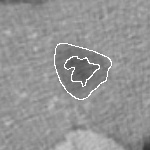
\includegraphics[width=0.2\textwidth]{scan_henbert/2008_09_16(2).jpg}
}
&
\subfloat[30 juin 2009 -- Jour 406]{\label{fig_hen_spatial_2}
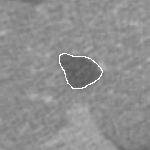
\includegraphics[width=0.2\textwidth]{scan_henbert/2009_06_30(2).jpg}
}&
\\
\subfloat[5 juill. 2010  -- Jour 776]{\label{fig_hen_spatial_3}
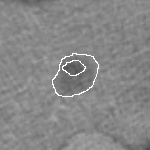
\includegraphics[width=0.2\textwidth]{scan_henbert/2010_07_05(3).jpg}
}&
\subfloat[25 oct. 2010 -- Jour 888]{\label{fig_hen_spatial_4}
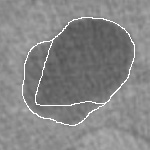
\includegraphics[width=0.2\textwidth]{scan_henbert/2010_10_25.jpg}
}&\\
\subfloat[7 janv 2011 -- Jour 962]{\label{fig_hen_spatial_5}
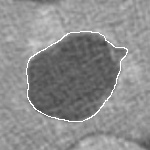
\includegraphics[width=0.2\textwidth]{scan_henbert/2011_01_07(2).jpg}
}&
\subfloat[10 juin 2011 -- Jour 1116]{\label{fig_hen_spatial_6}
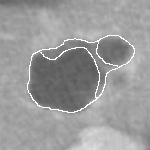
\includegraphics[width=0.2\textwidth]{scan_henbert/2011_06_10.jpg}
}&
\multirow{-3}{*}[105mm]{
 \subfloat[Aire tumorale. Chaque point représente l'aire de la tumeur mesurée sur les scanners et la ligne représente notre résultat numérique. \newline
Les lettres font référence aux scanners montrés sur la gauche. Les symboles 
 $\oplus$ représentent les tumeurs hétérogènes, {\large$\bullet$} les tumeurs plutôt homogènes et {\large$\circ$} les tumeurs pour lesquelles il est difficile de détecter sur le scanner un aspect hétérogène ou homogène dominant.  
Les valeurs des paramètres utilisés dans la simulation numérique sont données dans la  Table~\ref{table_param}.]{\label{fig:fit_area_henbert}
 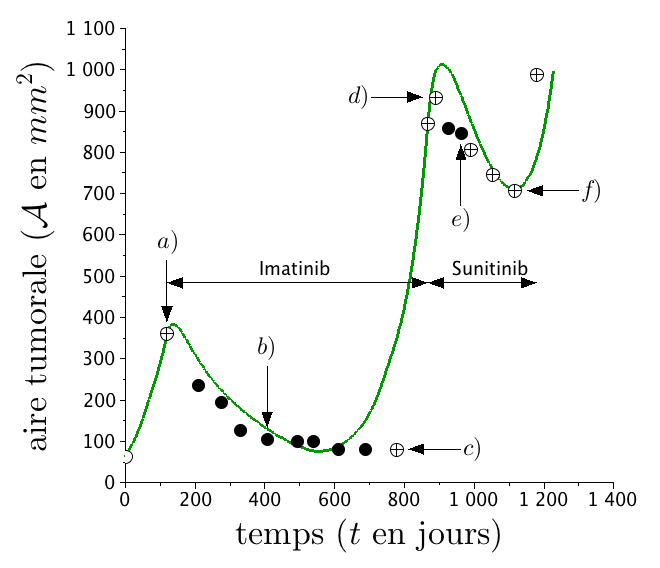
\includegraphics[width=0.59\textwidth]{fit_henbert_form3/henbert_area.png}
 }}
\end{tabular}
\caption{\label{fig_nber} Evolution spatiale de la métastase hépatique de \Nber sur une série de scanners.}
\end{figure}



Curieusement, juste avant les recroissances tumorales au Jour~776 (Figure~\ref{fig_hen_spatial_3})
et au Jour~1116 (Figure~\ref{fig_hen_spatial_6}), une couronne plus claire que le c\oe{}ur sombre apparaît, alors que la réponse au traitement se traduit par un assombrissement de la tumeur (\cf Figure~\ref{fig_hen_spatial_2} et~\ref{fig_hen_spatial_5}). 
De telles étapes successives de tumeurs homogènes/hétérogènes sont particulièrement prononcées dans les métastases hépatiques de GIST et notre but est de fournir une explication à ce type de comportement.


Le premier résultat de cet article est qu'il est possible de décrire l'évolution tumorale en terme d'aire tumorale comparable aux mesures réalisées sur les scanners, comme présenté sur la  Figure~\ref{fig:fit_area_henbert}; la ligne continue représentant notre résultat numérique. Il est important de noter que nous ne fournissons pas un modèle 1D qui décrit le volume tumoral. Nous traitons un modèle complexe d'EDPs non linéaires, qui est phénoménologique et qui décrit le comportement des cellules cancéreuses en fonction du temps et de l'espace. Par conséquent, le premier fit de l'aire tumorale n'est pas un résultat trivial.


Le second résultat est que notre modèle apporte de nouvelles informations sur la structure de la tumeur, ce qui semble corroborer par les scanners. En effet, comme présenté dans la suite, nous relions l'hétérogénéité tumorale à une augmentation de l'activité cellulaire signifiant qu'un phénotype résistant émerge dans la région plus claire. Selon notre modèle, de tels comportements peuvent être constatés avant la rechute effective, alors que le critère RECIST n'a pas changé. Par exemple, sur la Figure~\ref{fig:compare_spatial_nber}, 
nous comparons la structure de la tumeur à deux temps différents: l'hétérogénéité de la tumeur semble bien capturée par les simulations numériques. Ainsi, notre article peut être vu comme un premier pas dans le développement de nouveaux outils pour évaluer la réponse des tumeurs aux traitements  basés sur des inhibiteurs de tyrosine kinase.


\begin{figure}[h]
\subfloat[Jour 406]{
\raisebox{0.045\textwidth}{
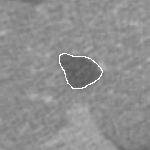
\includegraphics[width=0.19\textwidth]{scan_henbert/2009_06_30(2).jpg}}
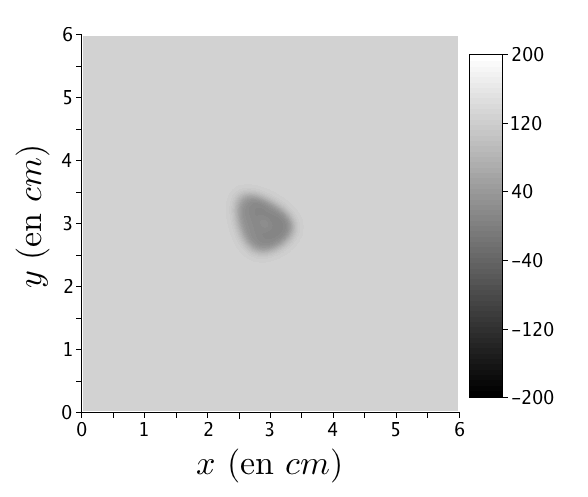
\includegraphics[width=0.3\textwidth]{fit_henbert_form3/vue_scan/vue_scan32.png}
}
\subfloat[Jour 776]{
\raisebox{0.045\textwidth}{
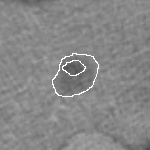
\includegraphics[width=0.19\textwidth]{scan_henbert/2010_07_05(3).jpg}}
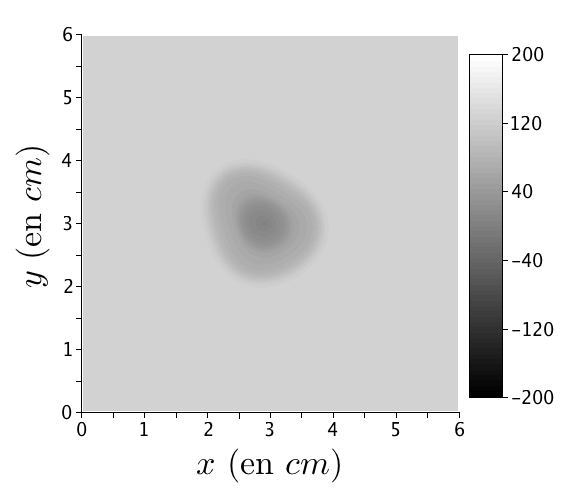
\includegraphics[width=0.3\textwidth]{fit_henbert_form3/vue_scan/vue_scan60.png}
}
\caption{\label{fig:compare_spatial_nber}
Comparaison entre les scanners du \Nber et les simulations numériques.
}
\end{figure}

\section{Description du modèle}

Notre modèle est un système d'EDPs similaire au modèle de 
Bresch {\it et al.}~\cite{Bresch2010}. Grosso modo, la tumeur est décrite grâce à des densités de cellules proliférantes et une densité de cellules cancéreuses nécrosées notées~$P$ et~$N$ respectivement. 
La prolifération cellulaire conduit à une augmentation de l'aire causée par une surpression dont le gradient transporte les cellules saines environnantes~$S$ loin du c\oe{}ur de la tumeur. 
Les cellules situées au centre de la tumeur se nécrosent à cause du manque d'oxygène, sauf si l'angiogenèse intervient pour leur apporter les provisions nutritives nécessaires.
L'angiogenèse et l'apport en nutriments sont pris en compte dans notre modèle via une description simpliste similaire à celle de~\cite{Fathallah2013,Billy2009545}: comme la vascularisation gouverne la concentration de nutriments parvenant à la tumeur, nous introduisons une variable~$M$ 
qui décrit à la fois la vascularisation, la néovascularisation et les nutriments apportés à la tumeur grâce à une équation d'advection-diffusion. 
Nous introduisons également les effets liés aux facteurs de croissance au travers de la variable~$\xi$ qui module~$M$. L'ensemble des quantités utilisées dans notre modèle est résumé dans la  Table~\ref{table_variable}.


La principale nouveauté réside en la modélisation des traitements. Deux traitements sont considérés (on peut voir dans \cite{lorz2013}, les récents travaux de Lorz~\etal\ pour des modèles plus élaborés sur les résistances aux traitements). 
Le premier est un inhibiteur de tyrosine kinase, comme l'imatinib, qui a un effet cytotoxique 
sur les cellules proliférantes. Le second est inhibiteur multi-kinases, comme le sunitinib ou le sorafenib, qui a un effet à la fois cytotoxique et antiangiogénique. En d'autres termes, en plus de l'effet cytotoxique, il bloque la production de facteurs de croissance, comme le facteur de croissance vasculaire endothélial (VEGF), et ainsi réduit la quantité de nutriments apportée à la tumeur. 
Il est bien connu que les médicaments cytotoxiques n'ont pas un impact similaire sur toutes les cellules cancéreuses métastatiques car des phénotypes résistants peuvent apparaître dans la population de cellules proliférantes. De plus les cellules cancéreuses peuvent résister différemment à l'hypoxie. Par conséquent nous découpons, comme dans~\cite{Bresch2009}, la densité~$P$ de cellules proliférantes en 3 sous-populations~$P_1$, $P_2$ et~$P_3$, telles  que~$P=P_1+P_2+P_3$, où
\begin{itemize}
\item $P_1$ représente la fraction de cellules proliférantes qui sont sensibles au premier traitement~$\TI$, basé sur la molécule d'imatinib, et sensible aussi au second traitement~$\TS$, à base de sunitinib ou de sorafenib, qui a un effet à la fois cytoxique et antiangiogénique. 
\item $P_2$ désigne la densité de cellules proliférantes qui sont résistantes à~$\TI$ et sensibles à~$\TS$,
\item $P_3$ représente les cellules proliférantes résistantes aux deux traitements. 
\end{itemize}

Il est important de noter que notre but n'est pas de décrire l'évolution de la tumeur depuis le tout début du GIST, mais de nous focaliser sur l'évolution des métastases situées dans le foie. 
Par conséquent, selon les observations cliniques, il semble pertinent de considérer que trois sous-populations sont présentes lorsqu'une métastase est détectée.
 \begin{table}[h]
 \rowcolors{2}{white}{gray!40}
 {\small
 \begin{tabular}{|l|l|l|}
 \hline
 \rowcolor[gray]{0.7} 
 Nom & Signification  & Unité \\
 \hline
 $P_1(t,\vecx)$ & Fraction de cellules proliférantes qui sont sensibles 
 aux traitements~$\TI$ et~$\TS$ & -  \\
% à~$\TI$ et à~$\TS$ & -  \\
 \hline
 $P_2(t,\vecx)$ & Fraction de cellules proliférantes qui sont résistantes à~$\TI$ et sensibles à~$\TS$  & -  \\
 \hline
 $P_3(t,\vecx)$ & Fraction de cellules proliférantes qui sont résistantes à~$\TI$ et à~$\TS$  & -  \\
 \hline
 $P(t,\vecx)$ & Fraction de cellules cancéreuses proliférantes (égale à~$P_1+P_2+P_3$) & -  \\
 \hline
 $N(t,\vecx)$ & Fraction de cellules nécrosées & - \\
 \hline
 $S(t,\vecx)$ & Fraction de cellules saines & - \\
 \hline
 $M(t,\vecx)$ & Fraction de nutriments // Vascularisation & - \\
 \hline
 $\xi(t)$ &Vitesse moyenne de transport des nutriments en direction de la tumeur & $cm.d^{-1}$ \\
 \hline
 $\vit(t,\vecx)$ &Vitesse du mouvement passif de la tumeur sous l'effet de la pression& $cm.d^{-1}$ \\
 \hline
 $\Pi(t,\vecx)$ & Pression du milieu\tablefootnote{
L'unité de masse dans la pression~$\Pi$ et la perméabilité~$k$ n'ont pas d'importance. Seule la quantité~$k\nabla\Pi$ est pertinente et ce terme est homogène à~$cm.d^{-1}$. 
Ainsi~$k$ et~$\Pi$ doivent juste avoir la même unité arbitraire de masse.}
 & $kg.cm^{-1}.d^{-2}$\\
 \hline
 \end{tabular}
 }
 \caption{\label{table_variable}Liste des quantités calculées par le modèle
 -- $d=\textrm{jour (day)}$ }
 \end{table}

\subsection{Le modèle mathématique}

Soit~$\Omega$ le domaine d'intérêt, où la tumeur croît, et soit~$\partial\Omega$ son bord, qui est supposé aussi régulier que nécessaire. Le domaine~$\Omega$ est supposé strictement inclus dans le tissu --le foie-- qui est plus grand. De plus, nous supposons que la tumeur n'atteint pas le bord~$\partial\Omega$.

\subsubsection{EDPs sur les cellules proliférantes, nécrosées et saines}

La densité de cellules proliférantes est gouvernée par l'équation de transport suivante~:
\begin{align}
\partial_t P_1 + \dive(\vit P_1) & =  \big(\gammapp(M)- \gammapd(M)\big)P_1 - \big(\muI \chiI (t)+\muS \chiS(t) \big)(1+M)P_1 & \ \textrm{ dans } \Omega, \label{eq_P1}\\
\partial_t P_2 + \dive(\vit P_2) & = \big(\gammapp(M)- \gammapd(M)\big)P_2 - \muS \chiS(t) (1+M)P_2 & \ \textrm{ dans }  \Omega, \label{eq_P2}\\
\partial_t P_3 + \dive(\vit P_3) & = (\gammapp(M) - \gammapd(M))P_3 & \ \textrm{ dans }  \Omega, \label{eq_P3}
\end{align}
où~$\chii(t)=\mathds{1}_{[\Tini{i},\rm \Tend{i}[}(t)$ est la fonction temps caractéristique du 
traitement~$\treat_{\rm i}$ et~$\mu_{\rm i}$ représente le taux de mortalité\footnote{Le taux de mortalité dû au traitement est clairement lié à la dose de médicament délivrée au patient, mais pas seulement. Par exemple la sensibilité du patient et la dose parvenant vraiment à la tumeur sont aussi impliquées.} causé par~$\treat_{\rm i}$ sur les cellules proliférantes, pour~$\rm i\in\{1,2\}$. 
Le terme~$\vit (t,\vecx)$ désigne la vitesse impliquée dans les changements d'aire de la tumeur et~$M(t,\vecx)$ représente la vascularisation et l'apport en nutriments. 
Le taux de prolifération (resp. de mortalité) des cellules proliférantes, noté~$\gammapp$ (resp.~$\gammapd$), dépend de~$M$ comme suit~:
\begin{align}
\gammapp(M) &=\gamma_0 \frac{1+\tanh\big(R(M-\Ms)\big)}{2}, \label{eq_gammapp}\\
\gammapd(M) &=\gamma_1 \frac{1-\tanh\big(R(M-\Ms)\big)}{2}, \label{eq_gammapd}
\end{align}
où~$R$ est un paramètre numérique régularisant\footnote{Notez que les fonctions~$\gammapp$ et~$\gammapd$ sont purement des fonctions de Heaviside régularisées. Pour les simulations numériques, nous fixerons arbitrairement~$R$ à 5.}, $\gamma_0$ et
$\gamma_1$ sont respectivement les paramètres de 
prolifération/mortalité et~$\Ms$ est le seuil d'hypoxie.


On suppose que les cellules saines sont uniquement sensibles à l'hypoxie, et qu'elles sont passivement transportées par les changements de l'aire tumorale~:
\begin{equation}
\partial_t S + \dive(\vit S) =  -\gammasd(M) S, \label{eq_S}
\end{equation}
où~$\gammasd$ est le taux de mortalité des cellules saines dû à l'hypoxie~:
\begin{equation}
\gammasd(M)=C_S \gamma_1  \max\Big(0,-\tanh\big(R(M-\Ms)\big)\Big). \label{eq_gammasd}
\end{equation}
Notez que~$\gammasd$  s'annule exactement si~$M\geq\Ms$ dans le but d'assurer que~$S=1$ sur le bord extérieur en tout temps. Finalement, la densité de cellules nécrosées satisfait la relation 
\begin{equation}\label{eq_N}
\partial_t N + \dive(\vit N) =  \gammapd(M) P +\gammasd(M) S  + \big(\muI \chiI(t)P_1 + \muS\chiS(t)(P_1+P_2)\big)(1+M) - \muN(1+M)N,
\end{equation}
où
\begin{equation}
P = P_1+P_2+P_3,
\end{equation}
et où~$\muN$ est un paramètre qui contrôle le taux d'élimination de la nécrose par le système immunitaire.

La condition suivante de Dirichlet est utilisée sur le bord si la vitesse est entrante~:
\begin{equation}\label{eq_CL_pop}
P_1=P_2=P_3=N=1-S=0  \quad \textrm{ pour } \vecx \in \partial \Omega, \textrm{ si } \vit.\nn<0,
\end{equation}
où~$\nn$ est le vecteur normal sortant au domaine~$\Omega$.
%%%%%%%%%%%%%%%%%%%%%%%%%%%%%%%%%%%%%%%%%%%%%%%%
\subsubsection{Fonctionnement}

En utilisant la condition de saturation suivante 
(comme dans~\cite{ambrosi2002})
\begin{equation}\label{eq_saturation}
P+N+S=1,
\end{equation}
et en sommant~\eqref{eq_P1},\eqref{eq_P2},\eqref{eq_P3},\eqref{eq_S} et~\eqref{eq_N},
on obtient 
\begin{equation}\label{eq_divv}
\dive \vit = \gammapp P - \muN (1+M)N.
\end{equation}
La loi de Darcy assure la solvabilité du système, de manière similaire à~\cite{Ribba2006532}:
\begin{equation}\label{eq_darcy}
\left\{
\begin{aligned}
\vit(t,\vecx) &=-k\nabla \Pi(t,\vecx) & \quad \textrm{ dans }  \Omega , \\
\Pi(t,\vecx) &=0 & \quad \textrm{ sur  } \partial \Omega,
\end{aligned}
\right.
\end{equation}
où~$\Pi$ est la pression (ou le potentiel) du milieu et~$k$ sa perméabilité. La condition de Dirichlet homogène, dans~\eqref{eq_darcy}, impose qu'en dehors de~$\Omega$, la pression du tissu sain n'est pas modifiée par la pression générée par la croissance tumorale. Cette hypothèse est valide pour de petites métastases n'impactant pas la forme du foie. En d'autres termes, la tumeur n'est pas mécaniquement contrainte par la région extratumorale. 


Observez qu'une condition de flux nul impliquerait nécessairement que~$\int_{\Omega} \gammapp P - \delta (1+M)N \textrm{\;d}\vecx $ s'annule en tout temps, ce qui n'est pas satisfait à~$t=0$.


Nous soulignons que notre article traite de métastases hépatiques de GIST et non de tumeurs primaires du foie. Par conséquent, les cellules métastatiques ne grandissent pas dans leur milieu d'origine~: elles ne peuvent pas infiltrer le foie mais leur prolifération induit une pression qui pousse les cellules saines vers l'extérieur. Pour ces raisons, nous choisissons une loi de Darcy pour décrire la croissance de la métastase. 


Bien sûr, une loi de Stockes ou n'importe quelle loi viscoélastique pourrait être utilisée, nous référons à~\cite{Bresch2009} et~\cite{ambrosi2002,byrne2003} pour plus de détails. De telles lois plus compliquées peuvent fournir une meilleure description du front tumoral. Cependant, le but de cet article n'est pas de fournir précisément le front tumoral~: notre objectif est de reproduire la structure interne de la métastase et non sa forme précise. 


%%%%%%%%%%%%%%%%%%%%%%%%%%%%%%%%%%%%%%%%%%%%%%%%
\subsubsection{Vascularisation, Nutriments et Angiogenèse}
Il reste à décrire l'apport de vascularisation/nutriments~$M$ 
et l'impact du traitement~$\TS$ sur celui-ci. Il est important de noter que la seconde ligne de traitement n'impacte pas directement~$M$, mais elle bloque la production de facteurs de croissance qui gouvernent la quantité~$M$.

Nous introduisons une variable scalaire~$\xi$, qui est associée à la moyenne de facteurs de croissance produits par les cellules cancéreuses. 
Il a été signalé dans~\cite{Holmes2007} que les cellules hypoxiques augmentent leur production de facteurs de croissance, tandis que les cellules hautement proliférantes n'ont pas besoin d'apports nutritifs supplémentaires. Ainsi, si~$M$ est en dessous du seuil~$\Ms$ alors~$\xi$ doit augmenter. 
Notez aussi que l'effet antiangiogénique du 
traitement~$\TS$ diminue la production
de~$\xi$, mais seulement pour les cellules~$P_1$ et~$P_2$ alors que~$P_3$ est la densité de cellules insensibles à~$\TI$ et~$\TS$. 
Nous décrivons ainsi l'évolution de~$\xi$ par
\begin{equation}\label{eq_xi}
\partial_t \xi = \alpha \int_\Omega \big(1+\epsilon_{\xi} - \gammapp(M) / \gamma_0 \big)\Big(\big(1-\nuS\chiS(t)\big)(P_1+P_2)+P_3\Big) \textrm{\;d}\vecx - \lambda \xi.
\end{equation}
Le paramètre adimensionné~$\nuS\in(0,1)$ représente l'effet antiangiogénique de~$\TS$, qui est supposé identique pour~$P_1$ et~$P_2$, et le paramètre~$\epsilon_{\xi}$ traduit la production minimale de facteurs de croissance par les cellules cancéreuses.


La quantité~$M$ décrit à la fois la vascularisation et la concentration de nutriments. Nous utilisons une équation de transport-réaction-diffusion pour décrire cette quantité~:
\begin{equation}\label{eq_M}
\left\{
\begin{aligned}
\partial_t M - \xi \frac{\nabla S}{\| \nabla S \|}\nabla M &= C_0 S
\left(1-\frac{M}{2\Ms}\right) - \eta PM +\psi \Delta M & \textrm{ dans } \Omega, \\
M(t,\vecx)&= 2\Ms & \textrm{ sur } \partial \Omega,
\end{aligned}
\right.
\end{equation}
où~$C_0$ est la capacité angiogénique des cellules saines, 
$\eta$ représente la destruction de la vascularisation par les cellules proliférantes, et~$\psi$ est un paramètre de diffusion.  
Le terme de transport~$\xi \frac{\nabla S}{\| \nabla S \|}. \nabla M$ de~\eqref{eq_M} décrit le fait que la vascularisation est apportée à la tumeur depuis le tissu sain qui est supposé bien vascularisé.  L'amplitude de la vitesse est égale à~$\xi$, qui représente le total des facteurs de croissance produit par les cellules proliférantes.


Le terme de diffusion décrit l'infiltration des vaisseaux sanguins et des nutriments dans la tumeur. D'un point de vue numérique, ce terme a un effet régularisant sur la vascularisation~$M$, et ainsi stabilise le modèle. 


Notez que si initialement 
\begin{align}\label{eq:borneM}
0\leq \|M|_{t=0}\|_{L^\infty}\leq 2\Ms
\end{align}
alors pour tout temps~$t$, $0\leq M(t) \leq 2\Ms$. Ceci traduit le fait que le tissu sain environnant est bien vascularisé et est fourni de suffisamment de nutriments.

\subsection{Formulation vectorielle des équations sur les cellules cancéreuses}

Pour simplifier les notations, considérons le vecteur des populations de cellules~$\W=\trans{(P_1, P_2, P_3, N)}$. On définit la fonction vectorielle 
$$
\medmuskip=1mu
\GG(M,\W) = \begin{pmatrix}
\Big(\gammapp(M)- \gammapd(M) - \big(\muI \chiI (t)+\muS \chiS(t) \big)(1+M)\Big) P_1 \\
\Big(\gammapp(M)- \gammapd(M) - \muS \chiS(t) (1+M)\Big)P_2 \\
\big(\gammapp(M) - \gammapd(M) \big)P_3 \\
\gammapd(M) P +\gammasd(M) (1-P-N)  + \big( \muI \chiI P_1 + \muS\chiS (P_1+P_2) \big) (1+M) - \muN(1+M)N
\end{pmatrix}.
$$
Il est également utile de définir~$\Frm(M,\W)$ comme
\begin{align}
  \label{eq_F}
  \Frm(M,\W):=\gammapp(M)\sum_{i=1}^3W_i-\muN(1+M)W_4,
\end{align}
de manière à réécrire l'ensemble d'équations~\eqref{eq_P1}-\eqref{eq_P3}, \eqref{eq_N} et~\eqref{eq_divv} fermés par la loi de Darcy de la manière suivante~:
\begin{equation}\label{eq_transport_pop}
\left\{
\begin{aligned}
\partial_t \W + (\nabla \W).\vit + \W (\dive \vit) &= \GG(M,\W) & \quad \textrm{ sur } & \Omega, \\
\W &=0 & \quad \textrm{ sur } & \partial \Omega \textrm{, si } \vit.\ \nn<0 ,
\end{aligned}
\right.
\end{equation}
et
\begin{equation}
\left\{ \begin{aligned}
 \label{eq_pression}
 -\dive\left(k\nabla \Pi\right) &=\Frm(M,\W), &\quad \textrm{ dans } & \Omega , \\
    \Pi(t,\vecx) &=0 & \quad \textrm{ sur  }& \partial \Omega.
\end{aligned}
\right. \end{equation}
Notez que la densité de cellules saines~$S$ est donnée par~\eqref{eq_saturation}.
\section{Méthodes numériques}\label{sec:NumMet}

Nous utilisons une méthode de volumes finis sur grille uniforme 2D. Pour la simulation numérique, le domaine~$\Omega$ est le 
rectangle~$[0,L]\times[0,D]$. Le domaine est maillé avec une grille cartésienne contenant~$N_x$ points sur l'axe~$x$ et~$N_y$ points sur l'axe~$y$.

Les densités de cellules cancéreuses sont discrétisées au centre des mailles et les vitesses sont discrétisées au milieu de chaque arête comme montré sur la Figure~\ref{fig:place_inconnues}.

\begin{figure}[h]
\centering
\setlength{\unitlength}{1.4mm}
\begin{picture}(100,50)

\rect{20}{10}{30}{30} %% \rect est defini dans mes macros

\multiput(16,10)(0,15){3}{\multiput(0,0)(1.5,0){26}{\line(1,0){0.5}}}
\multiput(20,6)(15,0){3}{\multiput(0,0)(0,1.5){26}{\line(0,1){0.5}}}

\multiput(20,25)(30,0){2}{\oval(4,2)}
\multiput(35,10)(0,30){2}{\oval(2,4)}
\rect{33.5}{23.5}{3}{3}
\put(6,27){$(i-\frac{1}{2},j)$}
\put(37,21){$(i,j)$}
\put(51,21){$(i+\frac{1}{2},j)$}
\put(36.5,42){$(i,j+\frac{1}{2})$}
\put(36.5,6){$(i,j-\frac{1}{2})$}

\put(15,5){\vector(1,0){9}}
\put(15,5){\vector(0,1){9}}
\put(14,15){$\ey$}
\put(25,4){$\ex$}

%% legende
\rect{63.5}{39.5}{3}{3}
\put(65,36){\oval(4,2)}
\put(65,31){\oval(2,4)}
\put(69,40){$P_1,P_2,P_3,N,S,M$}
\put(69,35){$v_x$}
\put(69,31){$v_y$}

\end{picture}
\caption{Discrétisation des inconnues sur une maille.\label{fig:place_inconnues}}
\end{figure}


Notez que l'égalité~\eqref{eq_saturation} donne directement~$S$, sans résoudre l'équation~\eqref{eq_S}. Le calcul est séparé en plusieurs étapes  (spliting), comme suit~:
\begin{itemize}
\item Etant donnés\footnote{L'exposant~$^n$ représente le temps discret~$t^n$ de la quantité 
(par exemple~$S^n$ est la densité de cellules saines au temps~$t^n$)}
$\W^n$ et~$M^n$ au temps~$t^n$, on infère~$\Frm^n=\Frm(M^n,\W^n)$ et
$\GG^n=\GG(M^n,\W^n)$.
\item On calcule d'abord la pression~$\Pi^n$ solution de~\eqref{eq_pression} avec~$F^n$ comme membre de droite, pression de laquelle on en déduit la vitesse~$\vit^n$ grâce à l'équation~\eqref{eq_darcy}.
\item Ensuite le nouveau temps~$t^{n+1}=t^n+\Delta t$ est déterminé en utilisant l'équation~\eqref{eq:dt}.
\item Après cela, $\W^{n+1}$ est calculé à partir de~\eqref{eq_transport_pop}, à partir duquel on infère~$S^{n+1}$.
\item On termine par le calcul de~$\xi^{n+1}$ et de~$M^{n+1}$ grâce à~\eqref{eq_xi}--\eqref{eq_M}.
\end{itemize}
Présentons maintenant dans le détail, les schémas utilisés dans les simulations numériques.

\subsection{Calcul de la vitesse et de la pression} 


Selon~\eqref{eq_divv} et~\eqref{eq_darcy}, 
la pression~$\Pi^n$ est donnée par
\begin{equation}\label{eq_pression_disc}
\left\{
\begin{aligned}
-\dive (k\nabla \Pi^n)&=\Frm^n:=\Frm(M^n,\W^n) & \quad \textrm{ sur } & \Omega , \\
\Pi^n &=0 & \quad \textrm{ sur } & \partial \Omega ,
\end{aligned}
\right.
\end{equation}
où~$\Frm$ est définie par~\eqref{eq_F}. 
Cette équation est résolue grâce à un schéma classique à 5-points. 
La composante de la vitesse selon~$\ex$, $v^{x,n}_{i+1/2 j}$ au point 
$\vecx_{i+1/2\,j}$ ({\it resp.} la composante selon~$\ey$, $v^{y,n}_{i,
  j+1/2}$ au point~${\vecx_{i\,j+1/2}}$) est donnée grâce à
\begin{equation*}
v^{x,n}_{i+1/2,j} = -k \frac{\Pi^n_{i+1,j}-\Pi^n_{i,j}}{\Delta x},\quad
v^{y,n}_{i,j+1/2} = -k \frac{\Pi^n_{i,j+1}-\Pi^n_{i,j}}{\Delta y}
\end{equation*}
et la vitesse~$\vit^n_{ij}$ au point~$\vecx_{ij}$ est approximée par
\begin{align}
  \label{eq_vit_discr}
  \vit^n_{ij}=    v^{x,n}_{ij}\ex
  +v^{y,n}_{ij}\ey=\frac{1}{2}\left(v^{x,n}_{i+1/2,j}
    +v^{x,n}_{i-1/2,j} \right) \ex+\frac{1}{2}\left(v^{y,n}_{i,j+1/2}
    +v^{y,n}_{i,j-1/2} \right) \ey.
\end{align}

\subsection{Equation d'advection}
Par la définition~\eqref{eq_F} de~$\Frm$, l'équation~\eqref{eq_divv} 
conduit à~$\dive\vit=\Frm$. 
Ainsi, l'équation~\eqref{eq_transport_pop} peut être écrite sous la forme non conservative
\begin{equation}\label{eq_non_conservative}
\partial_t \W + (\nabla \W).\vit = \Grm(M,\W)-(\dive \vit)\W = \Grm(M,\W)-\Frm(M,\W)\W,
\end{equation}
résolue grâce au spliting en temps suivant~:
\begin{align}
 \dfrac{\W^*-\W^n}{\Delta t / 2}  &= \GG^n-\Frm^n\W^n, %% & \textrm{then}
 \label{eq_snd_membre} \\
\dfrac{\W^\#-\W^*}{\Delta t} + (\nabla \W^*).\vit^n&= 0,%%& \textrm{then} 
 \label{eq_transp_weno}\\
 \dfrac{\W^{n+1}-\W^\#}{\Delta t / 2}  &= \GG^n-\Frm^n\W^n. \label{eq_snd_membre2} 
\end{align}
Cette forme non conservative est choisie dans le but de réutiliser les informations que nous possédons déjà sur la divergence de la vitesse, grâce à la relation~\eqref{eq_divv}.


Une méthode de type WENO5 comme donnée par~\cite{Liu1994} est utilisée pour approximer le gradient~$\nabla \W$ impliqué  dans~\eqref{eq_transp_weno}.
D'autres schémas d'ordre moins élevé ont aussi été essayés. Cependant la diffusion numérique de ces schémas est trop importante. Ceci conduit à une diffusion artificielle des nutriments dans la tumeur. La croissance tumorale est alors complètement modifiée par cet artefact. La résolution précise du transport est par conséquent un point important. De plus,  utiliser un schéma d'ordre élevé réduit, par le gain de convergence, les problèmes usuels liés à la résolution du problème non conservatif.

\subsection{Calcul des quantités~$\xi$ et~$M$}
L'équation scalaire~\eqref{eq_xi} est résolue grâce à la méthode classique d'Euler explicite~:
\begin{equation}\label{eq:xi_disc}
\dfrac{\xi^{n+1}-\xi^n}{\Delta t} = \alpha \int_\Omega \big(1+\epsilon_{\xi} - \gammapp(M^n) / \gamma_0 \big)\Big((P_1^n +P_2^n) \big(1-\nuS \chiS(t^n) \big)+P_3^n \Big) \textrm{\;d}\vecx - \lambda \xi^n,
\end{equation} 
où la formule standard des rectangles est utilisée pour approcher l'intégrale du membre de droite.


Pour résoudre l'équation d'advection-diffusion~\eqref{eq_M}
satisfaite par~$M$, le spliting en temps suivant est réalisé~:
\begin{align}
\dfrac{M^*-M^n}{\Delta t/2} &= C_0 S^n \left( 1-\dfrac{M^n}{2\Ms}\right) - \eta P^nM^n, %%& \textrm{then} 
\\
\dfrac{M^{\#}-M^*}{\Delta t} - \psi \dfrac{ \Delta M^\# + \Delta M^*}{2} &= \xi^n  \dfrac{\nabla S^n}{\| \nabla S^n \| }\nabla M^n, %%& \textrm{then} 
\label{eq_transp_diff_M}\\
\dfrac{M^{n+1}-M^\#}{\Delta t/2} &= C_0 S^n \left( 1-\dfrac{M^n}{2\Ms}\right) - \eta P^nM^n. \label{eq_snd_membre_M}
\end{align}
L'équation~\eqref{eq_transp_diff_M} est calculée comme une équation de la chaleur avec un schéma standard à 5 points de grille. Le membre de droite est approximé par un schéma de type WENO5.


\subsection{Le \twinweno~: un schéma WENO5 modifié}

Le schéma WENO5 standard comme donné par~\cite{Liu1994} est précis dans la plupart des cas, cependant certains ensembles de paramètres\footnote{L'ensemble de paramètre a été trouvé par incident en  fitant l'aire tumorale de \Chen, \cf Section~\ref{section chen}.} produisent des instabilités numériques (de telles instabilités ont aussi été constatées avec un schéma classique upwind). 
Plus précisément, partant d'une donnée initiale irrotationelle, la simulation numérique peut générer une structure en forme de trèfle, comme présenté sur la Figure~\ref{fig:simu_clover}, alors que la forme circulaire devrait être préservée. 
\begin{figure}[h!]
  \centering
  \subfloat[Jour 0]{\label{fig_chen_simu_spatial_1}
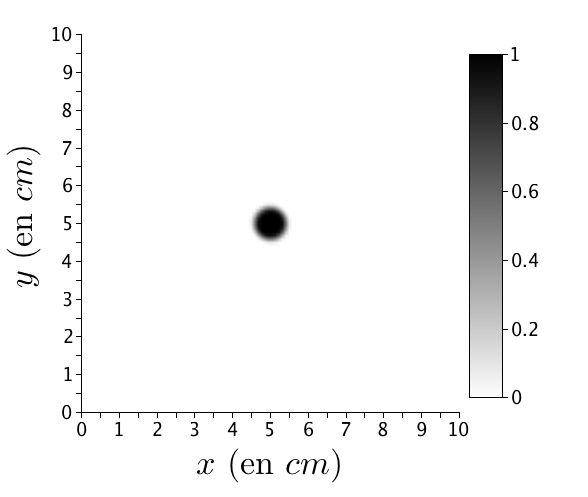
\includegraphics[width=0.3\textwidth]
{track_10x10_7/vue_S/1.png}}
\subfloat[Jour 543]{\label{fig_chen_simu_spatial_2}
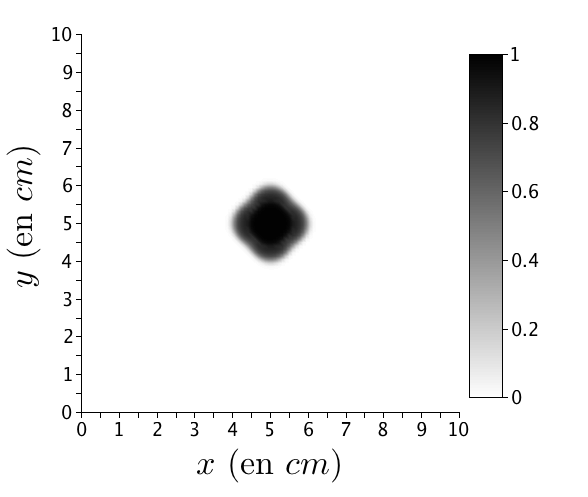
\includegraphics[width=0.3\textwidth]
{track_10x10_7/vue_S/34.png}}
\subfloat[Jour 1053]{\label{fig_chen_simu_spatial_4}
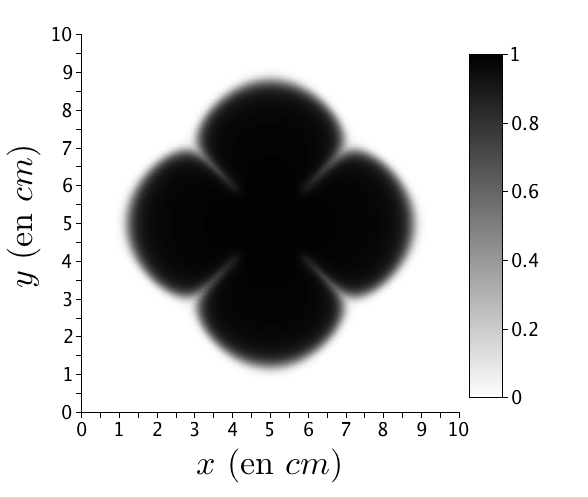
\includegraphics[width=0.3\textwidth]
{track_10x10_7/vue_S/65.png}}
\\
\subfloat[Profil de~$\vit_x$ le long de~$\ex$ au Jour 905]{\label{fig_vx_profile}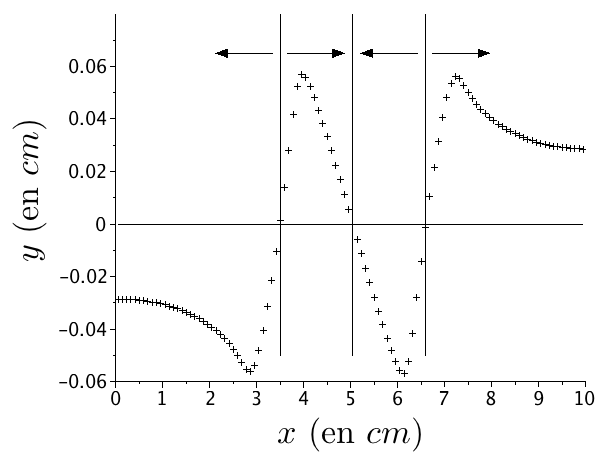
\includegraphics[width=.4\textwidth]
{track_10x10_7/coupe_vitesse_v2_56.png}}
\caption{Simulation numérique avec le stencil standard du WENO5 pour un jeu de paramètres spécifique. Partant d'une donnée initiale circulaire, une structure en forme de trèfle apparaît.} \label{fig:simu_clover}
\end{figure}

Notez que ce type d'erreur sur la forme conduit à une erreur sur l'évolution de l'aire de la lésion. En effet la forme de trèfle augmente la surface de contact ce qui modifie l'interaction entre la vascularisation et la tumeur. Ce type d'instabilités doit être fixé.
Le problème est dû au stencil du WENO5 qui tend à favoriser les directions du maillage lors de changement de direction de la vitesse.
Comme on peut le voir sur la Figure~\ref{fig_vx_profile}, 
au centre de la tumeur (autour de~$x=5\;cm$ sur la  Figure~\ref{fig_vx_profile}), il y a un point de compression~: 
la vitesse est centripète puisque~$v_x$ est positif à droite et négatif à gauche. 
De plus, aux alentours de~$1.5\;cm$ du centre de la tumeur, il y a une couronne de cellules proliférantes qui induit un mouvement d'étalement~: la vitesse est centripète près du centre mais centrifuge plus loin. 


Plus précisément, pour le schéma classique WENO5, en tout point 
~$\vecx_{ij}$ de la grille, l'approximation numérique 
$\W^{n+1}_{ij}$ de l'équation~\eqref{eq_transp_weno} au temps 
$t^{n+1}$ est donnée par
\begin{equation}\label{eq:WENO5}
\W^{n+1}_{i,j}=\W^n_{i,j} + \Delta t \Bigl(v_{i,j}^{x,n}
\mathcal{F}\left(\Delta x,(\W^n_{i+k,j})_{k=-3,\cdots, 3}\right) +
v_{i,j}^{y,n} \mathcal{F}\left(\Delta y,(\W^n_{i,j+k})_{k=-3,\cdots, 3}\right)\Bigr),
\end{equation}
où~$v_{i,j}^{x,n} $ et~$v_{i,j}^{y,n}$ sont définis par~\eqref{eq_vit_discr} et où~$\mathcal{F}$ est le fonction de flux WENO5 donnée par~\cite{Liu1994}. 
Pour éviter ces instabilités numériques, nous introduisons le schéma \twinweno, qui est la combinaison d'un WENO5 avec son stencil standard avec un autre WENO5 dont le stencil est une rotation d'angle~$\ang$ du premier (\cf Figure~\ref{fig:stencil_weno5_twin}), où~$\ang$ est défini en fonction des pas d'espaces de la grille, $\Delta x$ et~$\Delta y$, par 
 $$\ang=\arctan (\Delta y/\Delta x)\in (0,\pi/2). $$
\begin{figure}[h]
  \centering
\subfloat[Grille uniforme~$\thickmuskip=1mu  \Delta x=\Delta y$]{\setlength{\unitlength}{.8mm}
\begin{picture}(65,65)
\multiput(8,8)(0,8){8}{\line(1,0){56}}
\multiput(8,8)(8,0){8}{\line(0,1){56}}
\multiput(12,12)(8,0){7}{\multiput(0,0)(0,8){7}{\circle{2}}}
\multiput(12,36)(8,0){7}{\circle*{2}}
\multiput(36,12)(0,8){7}{\circle*{2}}
\multiput(12,12)(8,8){7}{\circle*{2}}
\multiput(12,60)(8,-8){7}{\circle*{2}}
\put(8,6){\vector(1,0){8}}
\put(6,8){\vector(0,1){8}}
\put(16,6){\vector(-1,0){8}}
\put(6,16){\vector(0,-1){8}}
\put(0,11){$\Delta y$}
\put(9,2){$\Delta x$}
\end{picture}}
\subfloat[Grille non-uniforme]{\setlength{\unitlength}{.8mm}
\begin{picture}(97,65)
\multiput(8,8)(0,8){8}{\line(1,0){84}}
\multiput(8,8)(12,0){8}{\line(0,1){56}}
\multiput(14,12)(12,0){7}{\multiput(0,0)(0,8){7}{\circle{2}}}
\multiput(14,36)(12,0){7}{\circle*{2}}
\multiput(50,12)(0,8){7}{\circle*{2}}
\multiput(14,12)(12,8){7}{\circle*{2}}
\multiput(14,60)(12,-8){7}{\circle*{2}}
\put(8,6){\vector(1,0){12}}
\put(6,8){\vector(0,1){8}}
\put(20,6){\vector(-1,0){12}}
\put(6,16){\vector(0,-1){8}}
\put(0,11){$\Delta y$}
\put(9,2){$\Delta x$}
\end{picture}}
\caption{Stencil du schéma \twinweno\ pour une grille uniforme (à gauche)
  et une grille non-uniforme (à droite).} \label{fig:stencil_weno5_twin}
\end{figure} 
Nous introduisons les coefficients~$(v^{r,n}_{i,j},
v^{\theta,n}_{i,j})$ et~$\Delta r$ définis par\footnote{Les coefficients~$v^{r,n}_{i,j}$
  et~$v^{\theta,n}_{i,j}$ sont définis de sorte que 
$$\vit^n_{i,j}=v^{x,n}_{i,j}\ex+v^{y,n}_{i,j}\ey=v^{r,n}_{i,j}\er+v^{\theta,n}_{i,j}\et,\quad\text{avec}\quad 
\er=\cos\ang\,\ex+\sin\ang\,\ey,\quad \et=-\sin\ang\,\ex+\cos\ang\, \ey.$$}
\begin{equation}
\begin{pmatrix}
v^{r,n}_{i,j} \\ v^{\theta,n}_{i,j}
\end{pmatrix} = \begin{pmatrix}
\cos \ang & \sin \ang \\ -\sin \ang & \cos \ang
\end{pmatrix} \begin{pmatrix}
v^{x,n}_{i,j} \\ v^{y,n}_{i,j}
\end{pmatrix}, \qquad  \Delta r=\sqrt{\Delta x^2+\Delta y^2},
\end{equation}
et nous discrétisons l'équation~\eqref{eq_transp_weno} grâce à notre schéma \twinweno\ : 
\begin{equation}\label{eq:twin-WENO5}
  \begin{split}
\W^{n+1}_{i,j} =\W^n_{i,j} &+ (1-\beta)\Delta t \Bigl(v_{i,j}^{x,n}
\mathcal{F}\left(\Delta x,(\W^n_{i+k,j})_{k=-3,\cdots, 3}\right) +
v_{i,j}^{y,n} \mathcal{F}\left(\Delta y,(\W^n_{i,j+k})_{k=-3,\cdots,
    3}\right)\Bigr)\\
&+\beta\Delta t \Bigl(v_{i,j}^{r,n}
\mathcal{F}\left(\Delta r,(\W^n_{i+k,j+k})_{k=-3,\cdots, 3}\right) +
v_{i,j}^{\theta,n} \mathcal{F}\left(\Delta r,(\W^n_{i-k,j+k})_{k=-3,\cdots, 3}\right)\Bigr),
  \end{split}
\end{equation}
où~$\beta\in(0,1)$ est un paramètre numérique que nous devons choisir. 
En particulier pour~$\beta=0$, on retrouve le WENO5 standard. 
Comme nous pouvons le voir sur la Figure~\ref{fig:compWENO5}, notre nouveau schéma préserve beaucoup mieux la propriété d'invariance par rotation dans les cas où le WENO5 ne la préserve pas.

\begin{figure}[!htb]
\subfloat[Jour 0]{\label{fig:correction_cross_spatial_1}
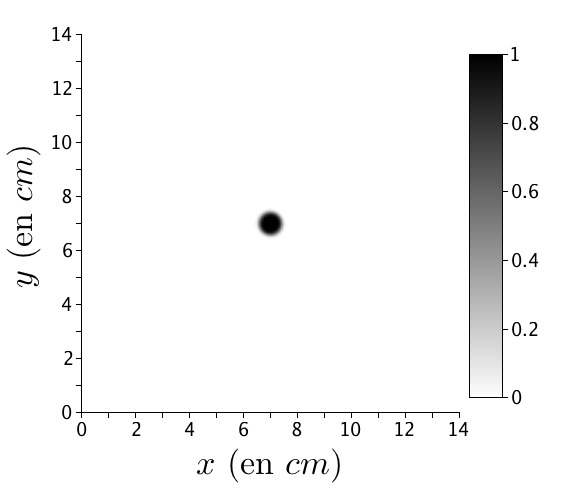
\includegraphics[width=0.33\textwidth]{track_14x14_cross/vue_S/1.png}}
\subfloat[Jour 543]{\label{fig:correction_cross_spatial_2}
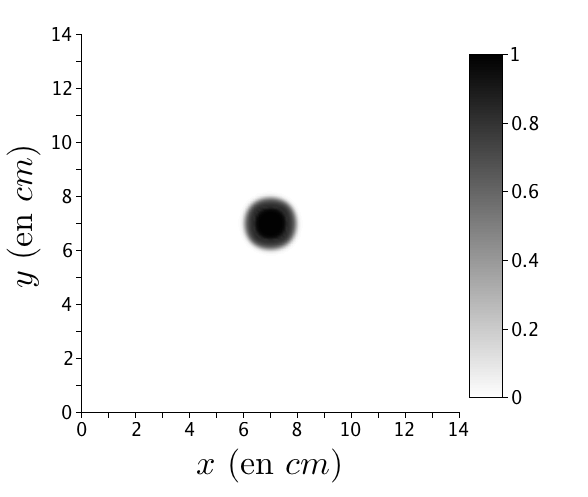
\includegraphics[width=0.33\textwidth]{track_14x14_cross/vue_S/34.png}}
\subfloat[Jour 1053]{\label{fig:correction_cross_spatial_3}
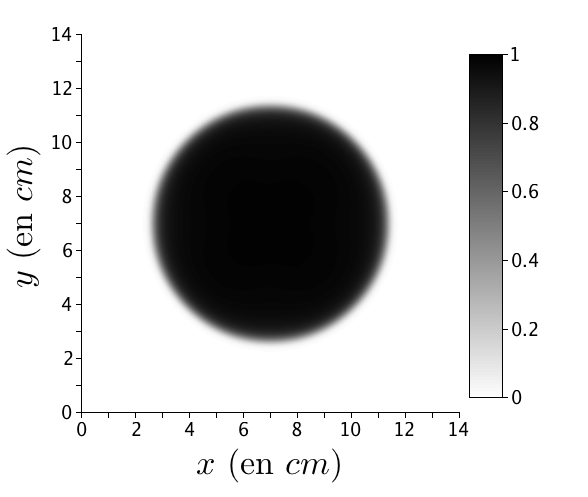
\includegraphics[width=0.33\textwidth]{track_14x14_cross/vue_S/65.png}}
\caption{Simulation numérique avec le schéma \twinweno\  ($\beta=0.26$).  
Comparé à la Figure~\ref{fig:simu_clover}, la conservation de l'invariance par rotation est très clairement améliorée. 
}\label{fig:compWENO5}
\end{figure}

\subsection{Condition CFL}

En outre, une restriction de type CFL est requise pour assurer la stabilité numérique. Tout d'abord, le schéma de type WENO5 conduit à une condition CFL qui s'écrit~:
\begin{equation}\label{eq:CFL-weno}
\Delta t < \min \left( \frac{\Delta x}{\max |v_x|} , \frac{\Delta y}{\max |v_y|}, \frac{\min(\Delta x , \Delta y )}{\xi}\right) := \Delta t_{adv}.
\end{equation}
Le schéma d'Euler explicite sur l'équation~\eqref{eq_snd_membre} conduit à l'inégalité 
(coordonnées par coordonnées)
$$
\W^{*}=\W^n+\frac{\Delta t}{2} (\GG^n -\Frm^n\W^n) \geq 
\left( \mathbf{1}+\frac{\Delta t}{2} (\bar{\GG}^n - \Frm^n\mathbf{1} )\right) \circ \W^n,
$$
où~$\mathbf{1}=\trans{(1,1,1,1)}$, le symbole~$\circ$ représente le produit d'Hadamard (multiplication terme à terme) et où~$\bar{\GG}^n$ vaut~:
$$
\bar{\GG}^n = \begin{pmatrix}
\gammapp(M^n)- \gammapd(M^n) - (\muI \chiI^n +\muS \chiS^n )(1+M^n) \\
\gammapp(M^n)- \gammapd(M^n) - \muS \chiS^n (1+M^n) \\
\gammapp(M^n) - \gammapd(M^n) \\
- \muN(1+M^n)
\end{pmatrix}.
$$
Une relation similaire entre~$\W^\#$ et~$\W^{n+1}$ 
peut être écrite depuis l'équation~\eqref{eq_snd_membre2}. 
Ainsi, en supposant que~$\W^n\geq 0$ et~$S^n=1-\Sigma_i W^n_i\geq 0$ 
au temps~$t^n$, la restriction suivante sur le pas de temps
\begin{equation}\label{eq:CFL-spliting-pop}
\Delta t < \min \left( \dfrac{1}{ \max_i \|  \bar{\GG}_i^n-\Frm^n \|_\infty} , \dfrac{1}{ \| \gammasd(M^n) + \Frm^n  \|_{\infty}} \right) := \Delta t_{W}.
\end{equation}
assure que~$\W^{n+1}\geq 0$ et~$S^{n+1}\geq 0$. 
De manière similaire, le schéma d'Euler explicite dans les équations~\eqref{eq:xi_disc} et~\eqref{eq_snd_membre_M} 
sur la vascularisation, conduit à
\begin{equation}\label{eq:CFL-spliting-vasc}
\Delta t < \min \left(  \frac{1}{\eta} , \frac{1}{\lambda}\right) := \Delta t_{angio}.
\end{equation}
Finalement, comme la vitesse peut être très petite, pour éviter les pas de temps 
$\Delta t$ trop larges, nous choisissons arbitrairement une vitesse~$\bar{\vit}$ et notre condition CFL s'écrit\footnote{Dans les simulations, nous choisissons 
$\bar{\vit}=1\;cm/mois$, en considérant~$30\;jours$ par mois et~$C_{\CFL}=0.4$.} 
\begin{equation}\label{eq:dt}
\Delta t =C_{\CFL}\min \left( \frac{1}{{\bar{\vit}}} \min( \Delta x, \Delta y) , \Delta t_{adv}, \Delta t_{W} , \Delta t_{angio} \right),
\end{equation}
pour une constante donnée~$C_{\CFL}<1$.

Notez qu'un schéma implicite aurait pu être utilisé pour relaxer les conditions~\eqref{eq:CFL-spliting-pop}-\eqref{eq:CFL-spliting-vasc}. 
Cependant avec l'ensemble de paramètres utilisé, le pas de temps est seulement limité par~$\Delta t_{adv}$, et cette condition reste aussi avec une méthode implicite. 

%%%%%%%%%%%%%%%%%%%%%%%%%%%%%%%%%%%%%%%%
\section{Résultats numériques}\label{sec:NumRes}

\subsection{Outils numériques pour comparer les résultats aux scanners}

Afin de comparer les résultats numériques aux scanners, nous devons définir des quantités d'intérêts appropriées aussi bien que développer un outil numérique qui reproduit l'échelle de gris. 
\subsubsection{Détermination numérique de l'aire tumorale, de la partie nécrosée et de la masse tumorale}

Soit le seuil~$\epsilon_{th}$, la fraction minimale de cellules tumorales en dessus de laquelle nous définissons numériquement la tumeur. 
L'aire tumorale, mesurée numériquement, s'écrit alors
\begin{equation}
\label{eq:airetot}
\mathcal{A}(t)=\int_\Omega \mathds{1}_{\{\vecx\;: P(t,\vecx)+N(t,\vecx) >\epsilon_{th}\}}(\vecx)\textrm{\;d}\vecx.
\end{equation}
On définit l'aire de chaque population cancéreuse par
\begin{equation}
\mathcal{A}_J(t)=\int_\Omega
\mathds{1}_{\{\vecx\,:\,J(t,\vecx)>\epsilon_{th}\}}(\vecx)\textrm{\;d}\vecx,
\qquad \text{pour}\quad J \in \{P_1,P_2,P_3,N \}.
\label{eq:airepop}
\end{equation}
On définit également la masse de chaque population, et la masse proliférante totale en tout temps par 
\begin{align}
\mathcal{M}_J(t)&=\int_\Omega J(t,\vecx) \textrm{\;d}\vecx, \quad J \in \{P_1,P_2,P_3,N \},
\label{eq:masspop} \\
\mathcal{M}(t)&=\int_\Omega P 
(t,\vecx)\textrm{\;d}\vecx.
\label{eq:masstot}
\end{align}


\subsubsection{Reconstitution numérique de scanners}

La comparaison de simulations numériques 
avec les scanners soulève une difficulté importante. 
Actuellement, contrairement aux simulations numériques qui fournissent en tout point chacune des quantités~$S$, $P$ et~$N$, les scanners fournissent des images en niveaux de gris reliés à la radiodensité locale grâce à l'échelle de 
Hounsfield. Comme les unités Hounsfield (HU) rendent possible de quantifier 
l'aire de la tumeur et de détecter sa localisation sur les scanners, nous introduisons une échelle numérique HU, qui est une combinaison linéaire de nos résultats numériques. 
Plus précisément, nous considérons une échelle linéaire de gris allant du noir au blanc. Pour chaque espèce (cellules proliférantes, saines et nécrosées), nous allouons les 
coefficients~$\tau_P$, $\tau_S$ et~$\tau_N$ à chacune de nos populations, et nous traçons ensuite la quantité
\begin{equation}\label{eq:grey_level}
\tau_P P + \tau_N N + \tau_S S,
\end{equation}
qui est une sorte d'échelle de niveau de gris numérique.
Comme pour les scanners abdominaux, l'échelle de Hounsfield est limitée de 
-200 à +200, nous fixons arbitrairement les coefficients ci-dessus à 
$$\tau_P=60,\quad \tau_S=120,\quad \tau_N=-140,$$
et nous associons à la valeur -200 la couleur noir, et à + 200 le blanc.


\subsection{Etude approfondie sur un patient spécifique}
\subsubsection{Comparaison des résultats numériques avec les données cliniques}
Nous nous focalisons à présent sur \Nber pour lequel nous avons aussi bien le protocole clinique complet que les données cliniques de l'évolution de l'aire tumorale et la séquence des scanners. 
Les simulations numériques sont réalisées dans un domaine carré de taille 
$L=D=6\;cm$ avec 120 points dans chaque direction. 
Le pas de temps~$\Delta t$ est calculé en utilisant l'équation~\eqref{eq:dt}. 


Les paramètres numériques ont été choisis de sorte à reproduire l'évolution de l'aire tumorale. En particulier, nous n'essayons pas de fiter avec les images, on vérifie seulement que l'évolution spatiale soit plausible comparée aux images médicales. Les paramètres sont résumés dans la Table~\ref{table_param}.

L'aire tumorale numérique est ensuite comparée aux aires mesurées sur la Figure~\ref{fig:fit_area_henbert} 
(les cercles représentent les données réelles, et la ligne pleine représente la simulation numérique). Il est important de noter que d'après cette 
figure, l'évolution de l'aire tumorale est bien reproduite. 
\begin{table}
\rowcolors{4}{white}{gray!40}
{\small
\begin{tabularx}{\textwidth}{|l|X|l|p{17mm}|p{17mm}|}
\hline
\rowcolor[gray]{0.7}  & & &  Valeur pour & Valeur pour \\
\rowcolor[gray]{0.7}  & & & le fit de  & le fit de \\
\rowcolor[gray]{0.7}  Nom & Signification & Unité & \Nber & \Chen \\
\rowcolor[gray]{0.7}  &   &  & (Figure~\ref{fig:fit_area_henbert}) & (Figure~\ref{fig:fit_area_chen})\\
\hline
\input{../data/params_value/table_fit.txt}
$\epsilon_{\xi}$ & Production résiduelle de facteur de croissance & - & 0.1 & 0.1 \\
\hline \hline \hline
$L,D$ & Dimensions du domaine de calcul &$cm$& 6 & 12 \\
$N_x,N_y$ & Nombre de points dans chaque dimension du \mbox{domaine} de calcul &-& 120 &132\\
$r_1$ & Rayon de la donnée initiale selon l'axe~$x$  & $cm$ & 0.47 & 0.5 \\
$r_2$ & Rayon de la donnée initiale selon l'axe~$y$ & $cm$ & 0.36 & 0.5 \\
$e$ & Sorte d'excentricité de la donnée initiale &-&0.35&0\\
$\beta$ & Poids du \Twinweno &-&0&0.3\\
\hline
\end{tabularx}
}
\caption{\label{table_param}Liste des paramètres du modèle et leur valeurs pour les deux patients considérés -- $d=\textrm{Jour (day)}$
}
\end{table}
Nous soulignons que la donnée initiale est cruciale dans la croissance de la tumeur. Afin de reproduire qualitativement la forme de la lésion au temps initial (\cf Figure~\ref{fig_hen_spatial_1}), 
la condition initiale est choisie comme une ellipse perturbée. 
Plus précisément, étant donnés 3 paramètres~$r_1$, $r_2$ et~$e$, nous définissons dans le domaine~$\Omega$, $d(\vecx)$ par
\begin{equation}\label{cond-ini}
d(\vecx)=\sqrt{\left(\dfrac{\mid x - L/2 \mid }{e\mid x - L/2 \mid +
      \crm r_1}\right)^2+\left(\dfrac{\mid y - D/2 \mid }{e\mid y -
      D/2 \mid + \crm r_2}\right)^2 },
\end{equation}
avec~$\vecx=(x,y)$ et où~$c=\dfrac{2\pi}{2\pi-\arccos(1-2\epsilon_{th})}$. 
La fonction~$Y$ definie par\footnote{Notez que si~$e=0$, alors~$Y$ est  invariant par rotation.}
\begin{equation}Y(\vecx)=\left\{
\begin{array}{ll}
1 & \textrm{si}\ d(\vecx)\leq 0.5,\\
0 & \textrm{si}\ d(\vecx)\geq 1, \\
\dfrac{1}{2}\Big(1-\cos \big(2\pi d(\vecx)\big)\Big)& \textrm{sinon},
\label{eq:CI_forme}
\end{array}\right.
\end{equation}
est ensuite utilisée afin d'imposer la condition initiale~:
\begin{equation}\label{eq:CI}
\begin{aligned}
P_1|_{t=0}&=(1-\Sigma_{ini})Y, \quad
P_2|_{t=0}=\dfrac{\Sigma_{ini}}{1+q_{ini}}Y, \quad
P_3|_{t=0}=q_{ini}P_2(t=0), \quad N|_{t=0}=0, \\
M|_{t=0}&=2\Ms,
\end{aligned}
\end{equation}
où~$\Sigma_{ini}$ représente la proportion de cellules résistantes au traitement~$\TI$ et~$q_{ini}$ est la proportion de cellules~$P_2$
qui sont aussi résistantes au traitement~$\TS$. Pour \Nber, nous avons choisi~$e=0.35$ et~$r_1=0.47$; $r_2=0.36$.


L'aspect spatial des simulations numériques présentées dans la Figure~\ref{fig:simu_henbert_scan}, fait apparaître les faits suivants~:
\begin{enumerate}[label=\roman*)]
\item \label{ini} Pendant la phase sans traitement, du jour~0
    au jour~119, la tumeur croît. Comme des cellules nécrosées et proliférantes sont présentes, les scanners numériques sont hétérogènes, comme on peut le constater Figure~\ref{fig_nber_simu_spatial_1}.
\item \label{TI} Ensuite le traitement~$\TI$ est administré du jour~119 au jour~867.
 Les cellules proliférantes~$P_1$ sont tuées et la nécrose devient prédominante. A cause du choix du coefficient~$\tau_N$, la tumeur numérique devient homogène et plus sombre comme le montre la Figure~\ref{fig_nber_simu_spatial_2}.
\item \label{failureTI} Le regain d'activité cellulaire au jour~776, juste avant la rechute, est caractérisé par une augmentation de l'hétérogénéité~: une couronne proliférante apparaît et recolonise progressivement l'intérieur nécrosé de la tumeur comme l'illustre la  Figure~\ref{fig_nber_simu_spatial_3}. Il est important de noter que le traitement~$\TI$ est encore administré et donc que les cellules résistantes commencent à devenir prédominantes.
\item \label{TS} Ensuite le traitement~$\TS$ est administré du jour~867 au jour~1298. Une fois de plus, la population nécrosée augmente et la tumeur numérique s'assombrit, comme le montrent les Figures~\ref{fig_nber_simu_spatial_4}-\ref{fig_nber_simu_spatial_5}.
\item \label{last} Finalement, au jour~1116, une nouvelle rechute se prépare. Ici encore, elle est caractérisée par une couronne proliérante au bord de la tumeur (\cf  Figure~\ref{fig_nber_simu_spatial_6}).
\end{enumerate}

Curieusement, les résultats numériques spatiaux sont en accord avec les données, au moins jusqu'au début de la dernière rechute autour du jour~1000. En fait, les cinq étapes que nous observons numériquement sont également constatées sur les scanners (\cf Figure~\ref{fig_hen_spatial_1}-\ref{fig_hen_spatial_6}).


Après le jour~1116, notre modèle n'est probablement plus valide car la structure de la tumeur numérique est très différente de celles des scanners. Peut-être que d'autres phénomènes qui ne sont pas pris en compte par notre modèle se produisent, comme les changements microenvironementaux ou d'autres mutations cellulaires. Des interactions dans la~$3^\textrm{ème}$ direction (non prise en compte ici) peuvent aussi être impliquées.

%%%%%%%%%%% Simu scan NBER
\begin{figure}[h]
\subfloat[Jour 119]{\label{fig_nber_simu_spatial_1}
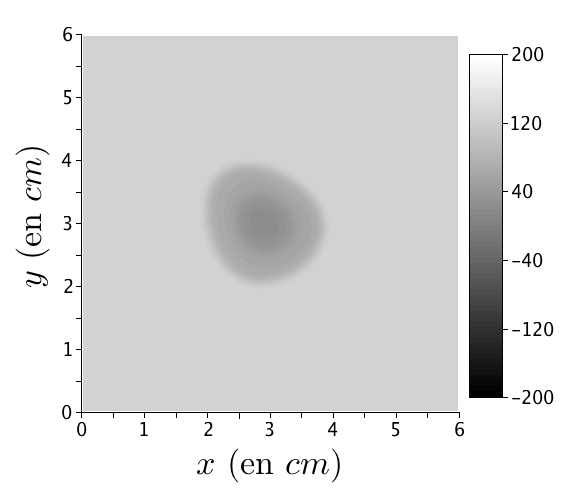
\includegraphics[width=0.32\textwidth]{fit_henbert_form3/vue_scan/vue_scan10.png}}
\subfloat[ Jour 409]{\label{fig_nber_simu_spatial_2}
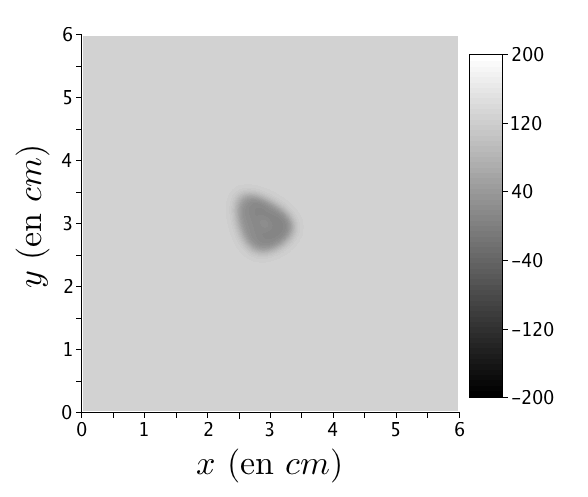
\includegraphics[width=0.32\textwidth]{fit_henbert_form3/vue_scan/vue_scan32.png}}
\subfloat[Jour 778]{\label{fig_nber_simu_spatial_3}
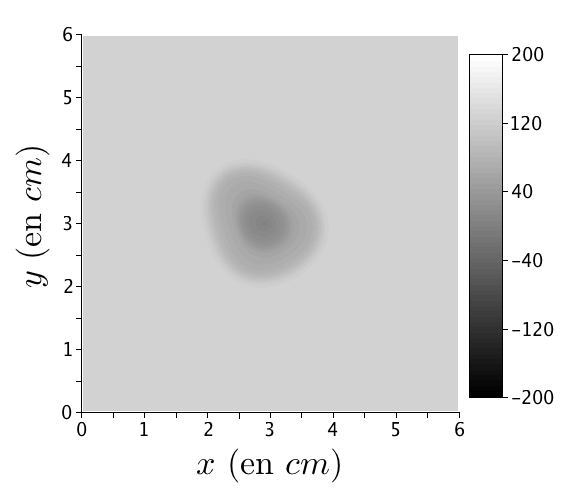
\includegraphics[width=0.32\textwidth]{fit_henbert_form3/vue_scan/vue_scan60.png}}\\
\subfloat[Jour 870]{\label{fig_nber_simu_spatial_4}
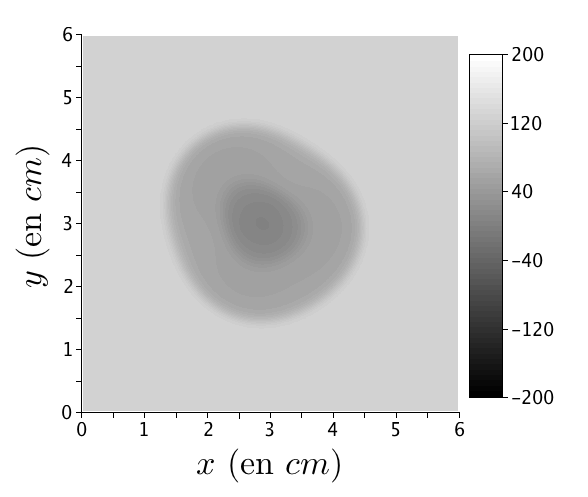
\includegraphics[width=0.32\textwidth]{fit_henbert_form3/vue_scan/vue_scan67.png}}
\subfloat[Jour 961]{\label{fig_nber_simu_spatial_5}
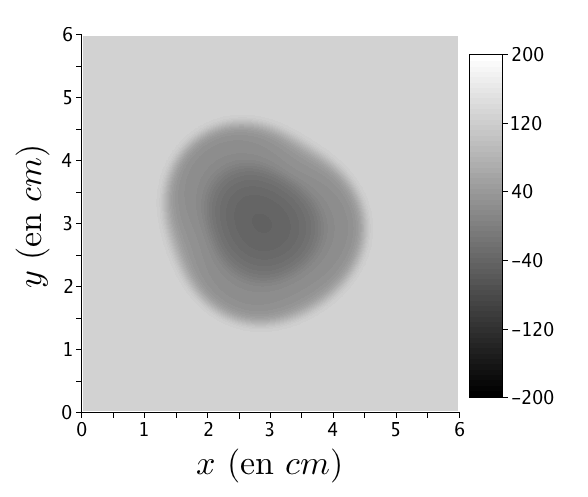
\includegraphics[width=0.32\textwidth]{fit_henbert_form3/vue_scan/vue_scan74.png}}
\subfloat[Jour 1120]{\label{fig_nber_simu_spatial_6}
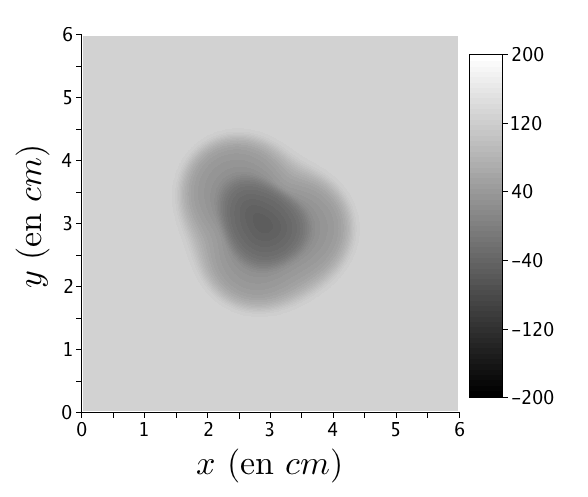
\includegraphics[width=0.32\textwidth]{fit_henbert_form3/vue_scan/vue_scan86.png}}
\caption{Simulation numérique pour \Nber~: évolution spatiale de la lésion avec reconstruction numérique de scanners.} \label{fig:simu_henbert_scan}
\end{figure}

Nous soulignons que le modèle semble fournir d'importantes informations auxquelles les cliniciens n'ont pas accès avec les dispositifs d'imagerie. Plus précisément, la  Figure~\ref{fig:simu_henbert_mass_area} qui présente l'évolution de l'aire et de la masse  de  \emph{chaque} population de cellules, nous permet de dire que selon notre modèle~: 
\begin{itemize}
\item Pendant le premier rétrécissement de la tumeur causé par le 
traitement~$\TI$, du jour~119 au jour~406, on observe que
\begin{enumerate}[label=\roman*)]
\item Le traitement~$\TI$ tue les cellules proliférantes~$P_1$ qui deviennent du tissu nécrosé. 
\item La réduction de l'aire est due à l'élimination de la nécrose par le système immunitaire. 
\item Les populations de cellules~$P_2$ et~$P_3$ qui ne sont pas sensibles au traitement~$\TI$ continuent de se diviser.
\end{enumerate}
\item Pendant plusieurs mois, du jour~406 au jour~778, l'aire tumorale continue de décroître lentement à cause de la mort de la population~$P_1$. Cependant les populations de cellules~$P_2$ et~$P_3$ continuent de grandir et prennent progressivement la place des cellules nécrosées éliminées.  Même si l'activité cellulaire de~$P_2$ et~$P_3$ n'est pas affectée par le traitement, il conduit dans un premier temps à une stabilisation de l'aire tumorale avant la recroissance au 
jour~778. En fait, quand~$P_2+P_3$ devient trop grand, la croissance de l'aire tumorale reprend et est gouvernée par les cellules résistantes au traitement~$\TI$.
\item Pendant le traitement~$\TS$, du jour~867 au jour~1298, nous pouvons remarquer que 
\begin{enumerate}[label=\roman*)]
\item La population~$P_1$ est encore sensible au traitement. 
\item La population~$P_2$, sensible au traitement~$\TS$, se nécrose.
\item La population~$P_3$ qui est résistante aux deux traitements continue de croître.
\end{enumerate}
\end{itemize}

\begin{figure}[h]
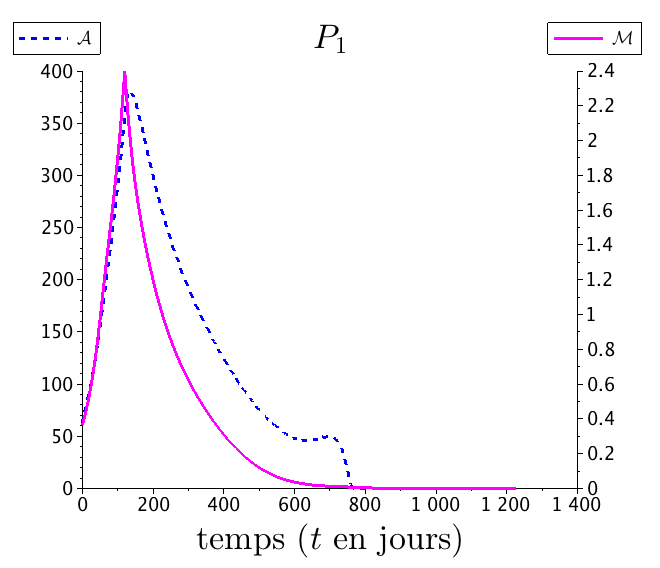
\includegraphics[width=0.32\textwidth]{fit_henbert_form3/P1.png} 
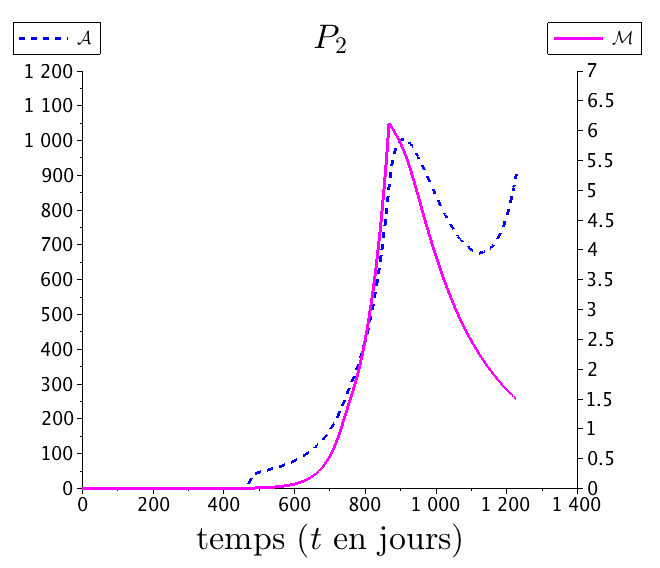
\includegraphics[width=0.32\textwidth]{fit_henbert_form3/P2.png} 
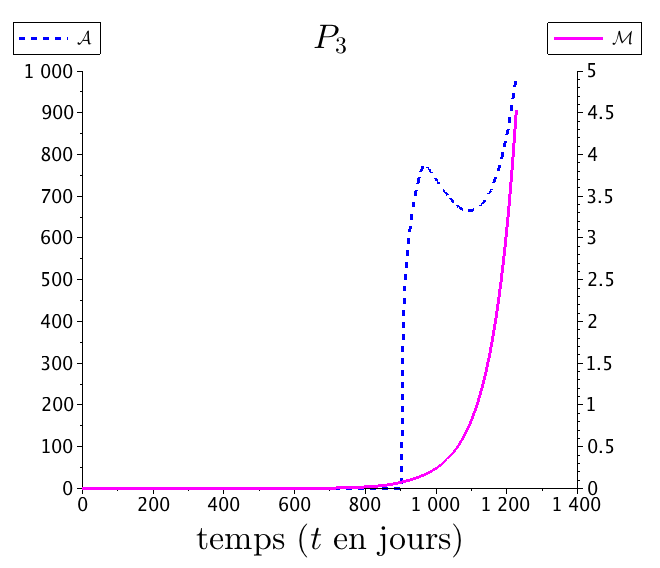
\includegraphics[width=0.32\textwidth]{fit_henbert_form3/P3.png}\\
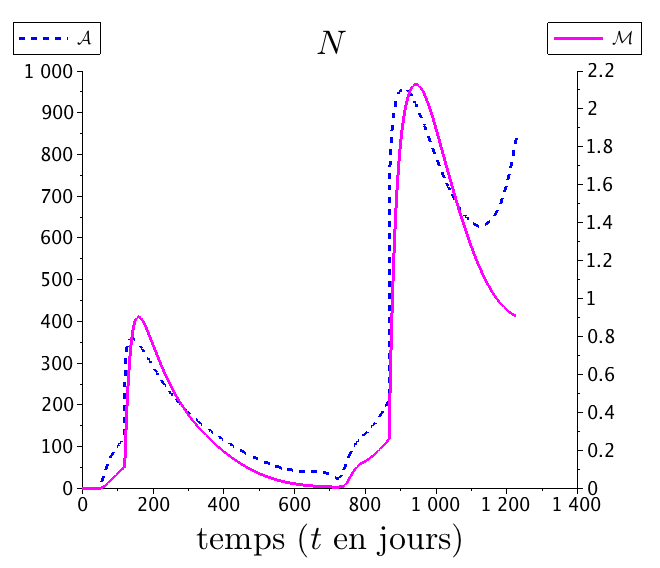
\includegraphics[width=0.32\textwidth]{fit_henbert_form3/N.png} 
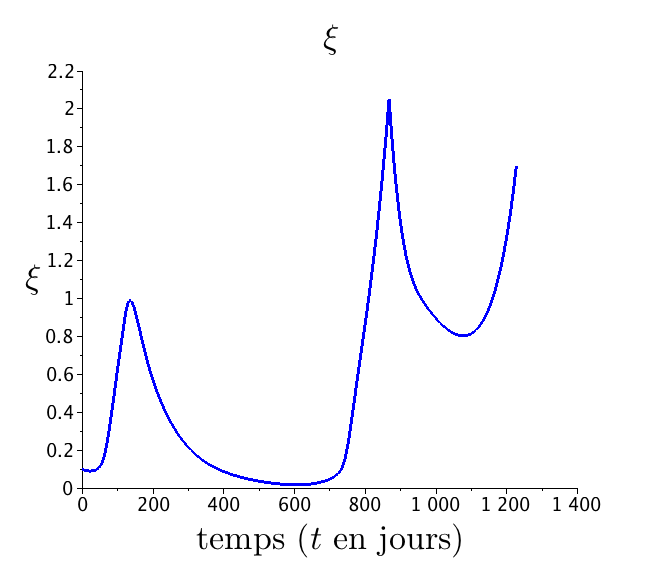
\includegraphics[width=0.32\textwidth]{fit_henbert_form3/xi.png} 
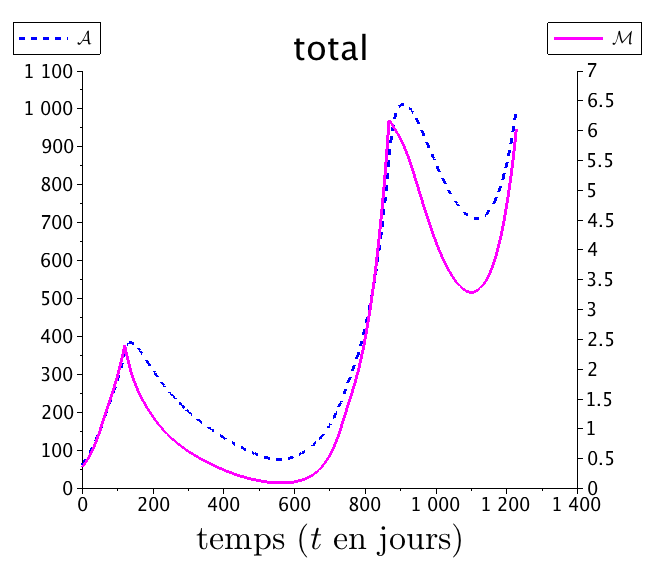
\includegraphics[width=0.32\textwidth]{fit_henbert_form3/total.png}
\caption{Evolution de la masse (intégrale du niveau de gris, dans une unité arbitraire) et de l'aire ($mm^2$) de chaque population de cellules et évolution du signal angiogénique ($cm.d^{-1}$) données par les simulations numériques.} \label{fig:simu_henbert_mass_area}
\end{figure}

Il est important de noter que pour chaque rechute, l'activité proliférante reprend sur le pourtour de la tumeur, là où sont présents les nutriments. 
De plus, notre modèle présente des différences entre l'évolution de l'aire tumorale~$\mathcal{A}$ et l'évolution de la masse tumorale~$\mathcal{M}$ données respectivement par~\eqref{eq:airetot} et~\eqref{eq:masstot}. 

En particulier, la masse de cellules cancéreuses décroît juste après l'administration du traitement alors que l'aire tumorale décroît avec un retard. 
Ce délai est dû au fait que les cellules proliférantes tuées basculent dans une phase nécrosée. Ainsi l'aire tumorale reste la même jusqu'à ce que le système immunitaire élimine cette nécrose. 
De plus, notre modèle permet de distinguer les effets des deux traitements sur l'angiogenèse. 
En effet, le traitement~$\TS$ inhibe directement le signal angiogénique alors que le  traitement~$\TI$ tue la population~$P_1$, ce qui implique indirectement une diminution de la production du signal.


\subsubsection{Etude numérique de l'influence de l'efficacité du traitement~$\TI$}\label{subsec:NumEff}
Nous nous intéressons ici, à l'étude numérique de différents aboutissements obtenus avec le 
traitement~$\TI$ afin d'examiner son influence sur la croissance tumorale. 
Prenons les paramètres de la Table~\ref{table_param}, et faisons juste varier~$\muI$. 
Définissons deux durées caractéristiques~:
\begin{itemize}
\item $\TPFS$ (progression-free survival time) qui est le temps de survie sans aggravation. C'est le temps pour lequel la taille de la tumeur reste inférieure à sa taille au début du traitement.  
\item $\Td$, qui est le temps de doublement. C'est la durée pour laquelle l'aire tumorale reste inférieure au double de sa taille initiale au début du traitement. 
\end{itemize}
 %%%%%%% Figure variation dose traitement
\begin{figure}[!htb]
\subfloat[Temps de survie sans aggravation ($\TPFS$ en jours) en fonction de~$\muI$.]{
\label{fig:Tmaintien_nber}
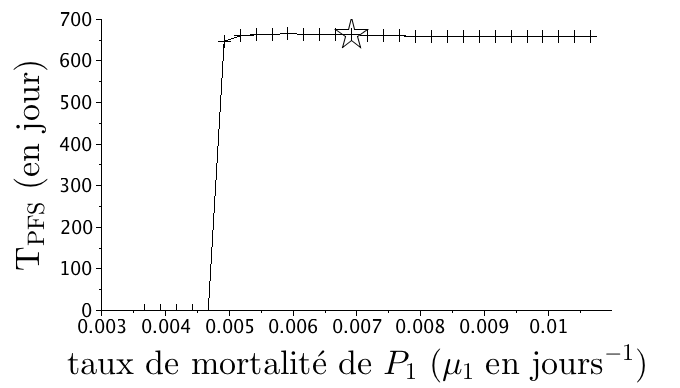
\includegraphics[width=0.48\textwidth]{DB-nber-eff-glivec/Tmaintien.png}}
\subfloat[Temps de doublement ($T_{double}$ en jours) en fonction de~$\muI$.]{
\label{fig:Tdouble_nber}
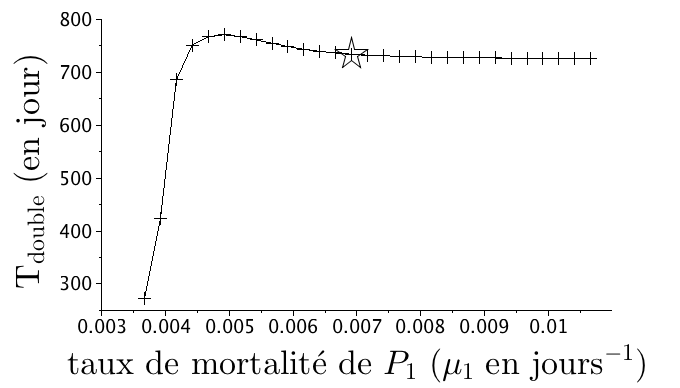
\includegraphics[width=0.48\textwidth]{DB-nber-eff-glivec/Tdouble.png}}\\
\subfloat[Aire minimale atteinte ($\Amin$ en~$mm^2$) en fonction de~$\muI$.]{
\label{fig:Amin_nber}
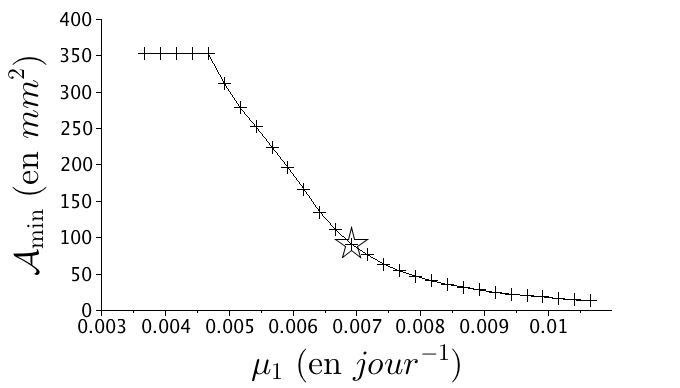
\includegraphics[width=0.48\textwidth]{DB-nber-eff-glivec/Amin.png}}
\subfloat[Portrait de phase.]{
\label{fig:portrait_phase_nber}
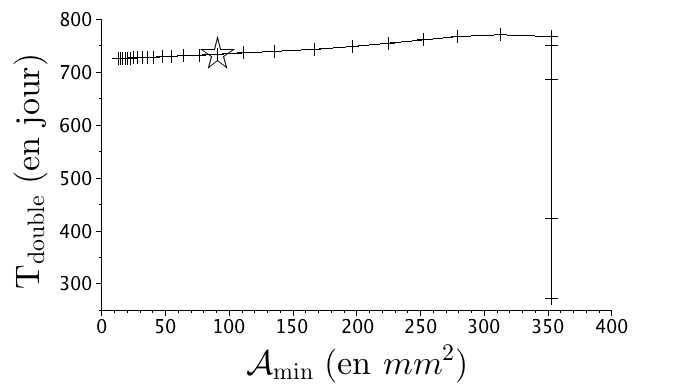
\includegraphics[width=0.48\textwidth]{DB-nber-eff-glivec/portrait_phase.png}}
\caption{Efficacité du traitement~$\muI$ sur \Nber. Les étoiles correspondent aux paramètres utilisés dans la Figure~\ref{fig_nber} pour le fit de l'aire tumorale. \label{fig:eff_glivec_nber}}
\end{figure}


Notez que cette étude est purement théorique et ne peut pas être utilisée telle quelle pour l'optimisation de traitement car l'évolution complète de la maladie (phases de rechute incluses) est nécessaire pour calibrer les paramètres utilisés dans les simulations. Par conséquent, il est clair que notre approche ne peut pour l'instant pas conduire à une détermination d'un protocole optimal de traitement, mais cette étude numérique est déjà un premier pas crucial au vue de l'importance de l'enjeu.


Sur la Figure~\ref{fig:Tmaintien_nber} est présenté le temps de survie sans aggravation~$\TPFS$ en fonction de~$\muI$. 
Si~$\muI$ est en dessous une valeur seuil~$\mu_{th}$ ($\mu_{th}\sim 0.0047$ pour \Nber), alors la croissance tumorale n'est pas stoppée.  
Pour~$\muI$ en dessus de ce seuil, $\TPFS$ augmente rapidement et atteint un plateau, ce qui signifie qu'il n'est pas nécessaire d'augmenter la dose puisque cela n'aurait pas d'effet sur  le temps de survie sans aggravation~$\TPFS$.

Sur la Figure~\ref{fig:Tdouble_nber} est présenté le temps de doublement~$\Td$. 
Comme nous pouvons le voir, $\Td$ n'augmente pas avec l'augmentation de la dose au-delà du seuil~$\mu_{th}$, ce qui signifie une fois de plus qu'il n'est pas nécessaire d'augmenter la dose au-delà d'une certaine valeur seuil.


L'aire minimale atteinte par la tumeur en fonction de~$\muI$ est présentée sur la Figure~\ref{fig:Amin_nber}. Notez que la courbe est décroissante~: en effet plus~$\muI$ est élevé, plus l'aire minimale atteinte est petite. Cependant, comme le montre la  Figure~\ref{fig:portrait_phase_nber}, la relation entre la taille minimale et le temps de doublement n'est pas monotone. En particulier, si la taille minimale est très petite, alors le temps de doublement peut être plus petit.  
Ceci peut être dû à des mécanismes de sélection darwinienne~: 
la population~$P_1$, qui est prédominante lorsque la lésion est détectée, est tuée plus vite par le traitement et ainsi plus de place et de nutriments sont disponibles pour la croissance des populations résistantes~$P_2$ et~$P_3$. Ainsi le temps de doublement devient plus court. 
Ces courbes montrent qu'il existe un seuil~$\mu_{th}$ à partir duquel le traitement~$\treat_1$ est efficace. Au-delà de ce seuil, l'aire minimale atteinte par la tumeur décroît, mais le temps de survie du patient n'augmente pas.

\section{Discussion}
Dans la section précédente, nous avons étudié en détail notre modèle sur un patient spécifique, \Nber, dont la lésion tumorale a été suivie par une série de scanners. Nous avons trouvé les paramètres qui rendent possible la comparaison qualitative des images médicales avec les images numériques, grâce à notre reconstitution numérique de scanners, et nous avons également fité l'aire tumorale. La lésion du patient est intéressante car elle est confinée à l'intérieur du foie, et donc son évolution n'est pas mécaniquement contrainte par l'organe. 
Cependant, dans certains cas, la métastase est proche du bord du foie. Dans de tels cas, il n'y a pas d'espoir de produire des résultats quantitatifs sur l'évolution spatiale de la lésion, mais dans la section suivante, nous montrerons que l'évolution de l'aire tumorale peut être correctement décrite.
\subsection{Evolution de l'aire tumorale de \Chen}\label{section chen}
Dans cette section, on s'intéresse à \Chen, dont l'évolution tumorale est assez différente de celle \Nber. En effet le protocole clinique de ce patient est le suivant~:
\begin{enumerate}[label=\roman*)]
\item \Chen est traité dans un premier temps avec un inhibiteur de tyrosine kinase mono-cible (imatinib), qui stabilise l'aire de la tumeur pendant plus de 10 mois avant une rechute. 
\item Le sunitinib, inhibiteur de tyrosine kinase multi-cibles, est démarré mais contrairement à \Nber, il est totalement inefficace. 
\item Un troisième traitement est administré. Le sorafenib est un autre inhibiteur de tyrosine kinase multi-cibles, qui a à la fois un effet cytotoxique et antiangiogénique. La tumeur semble être sensible à ce médicament pendant plusieurs mois jusqu'à ce qu'une nouvelle rechute arrive. 
\end{enumerate}
Malheureusement, comme illustré par la Figure~\ref{fig:fit_area_chen}, l'évolution tumorale est très rapide entre le scanner du jour~429 et celui de jour~845 sur lequel la métastase a atteint le bord du foie, et ainsi, avec notre modèle nous n'avons pas espoir de fournir une croissance tumorale numérique qui soit spatialement en accord avec les scanners car les effets de bord de l'organe devraient être pris en compte. Par conséquent, nous nous intéresserons à la l'aire tumorale comme donnée par les cliniciens, le principal enjeu ici étant de capter une croissance aussi rapide. 

\begin{figure}[h]
\captionsetup[subfigure]
{margin={10pt,10pt}}
\begin{tabular}{@{\hspace{-7mm}}ccc}
\setlength{\unitlength}{0.01\textwidth}
\subfloat[23 mai 2007 -- Jour 0]{\label{fig_chen_spatial_1}
\begin{picture}(20,20)
\put(0,0){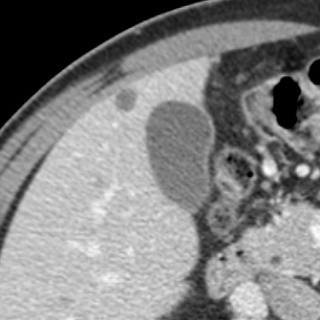
\includegraphics[width=0.2\textwidth]{scan_chen/2007_mai_23.jpg}}%
\linethickness{.8mm}
\put(5,5){\vector(1,3){2.5}}
\end{picture}
}&
\subfloat[25 juill. 2008 -- Jour 429]{\label{fig_chen_spatial_2}
\setlength{\unitlength}{0.01\textwidth}
\begin{picture}(20,20)
\put(0,0){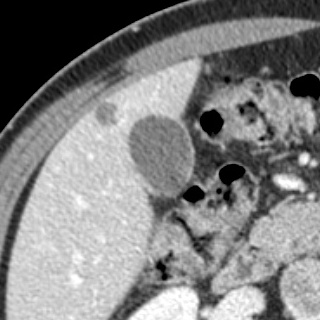
\includegraphics[width=0.2\textwidth]{scan_chen/2008_juil_25.jpg}}%
\linethickness{.8mm}
\put(3.9,4.2){\vector(1,3){2.5}}
\end{picture}
}&\\
\subfloat[14 sept. 2009 -- Jour 845]{\label{fig_chen_spatial_3}
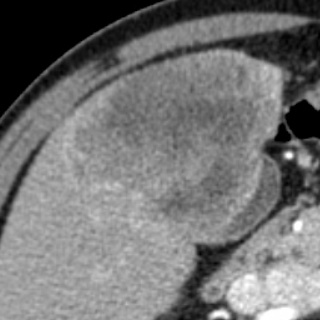
\includegraphics[width=0.2\textwidth]{scan_chen/2009_sept_14.jpg}%
}&
 \subfloat[6 avril 2010 -- Jour 1049]{\label{fig_chen_spatial_4}
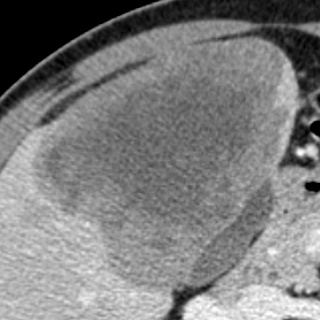
\includegraphics[width=0.2\textwidth]{scan_chen/2010_avril_06.jpg}%
 }&\\
 \subfloat[28 sept. 2010 -- Jour 1224]{\label{fig_chen_spatial_5}
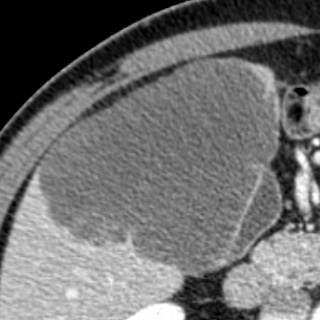
\includegraphics[width=0.2\textwidth]{scan_chen/2010_sept_28.jpg}%
 }&
 \subfloat[20 mai 2011 -- Jour 1458]{\label{fig_chen_spatial_6}
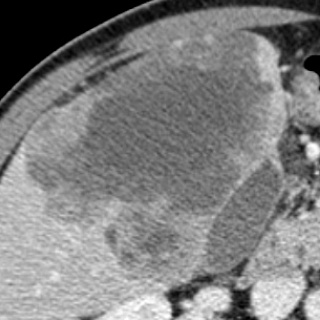
\includegraphics[width=0.2\textwidth]{scan_chen/2011_mai_20.jpg}%
 }&
\multirow{-3}{*}[105mm]{
\subfloat[Aire tumorale. Chaque point représente l'aire de la tumeur mesurée sur les scanners et la ligne représente notre résultat numérique. \newline
Les lettres font référence aux scanners montrés sur la gauche. Les symboles 
 $\oplus$ représentent les tumeurs hétérogènes, {\large$\bullet$} les tumeurs plutôt homogènes et {\large$\circ$} les tumeurs pour lesquelles il est difficile de détecter sur le scanner un aspect hétérogène ou homogène dominant.  
Les valeurs des paramètres utilisés dans la simulation numérique sont données dans la Table~\ref{table_param}.]{\label{fig:fit_area_chen} 
 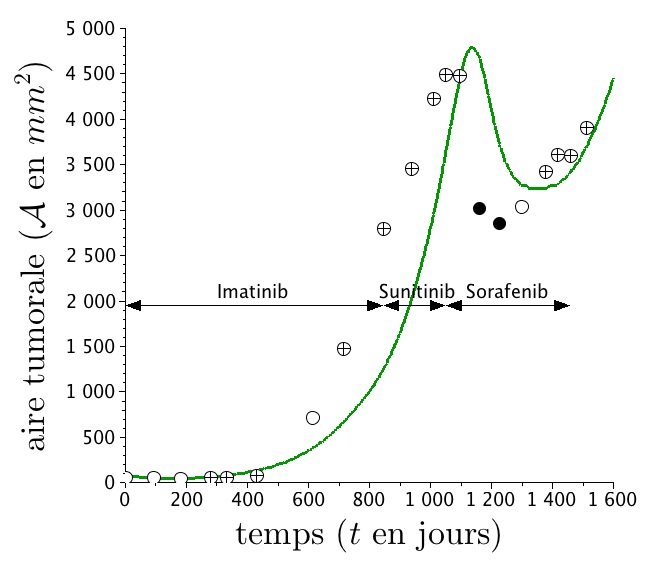
\includegraphics[width=0.59\textwidth]{chen_area.png}
 }}
\end{tabular}
\caption{\label{fig_chen_spatial} Evolution spatiale de la métastase hépatique de \Chen sur une série de scanners. Nous examinons l'évolution de la lésion\protect\footnotemark~située au départ en haut à gauche de la Figure~\ref{fig_chen_spatial_1}.}
\end{figure}
\footnotetext{Ne pas confondre la métastase avec la vésicule biliaire qui est plus grosse sur les deux premiers scanners.}


Comme le sunitinib est totalement inefficace dans ce cas, nous considérons que le 
traitement~$\TI$ est administré du jour~0 au jour~845, tandis que le 
traitement~$\TS$, basé sur le sorafinib, est administré du jour~1049 au jour~1600. 
Nous avons trouvé des paramètres qui rendent possible la comparaison qualitative entre l'aire tumorale mesurée par les cliniciens et notre aire tumorale numérique. Ces paramètres sont donnés dans la  Table~\ref{table_param}. 
La donnée initiale a été choisie invariante par rotation, en accord avec les données de la 
Figure~\ref{fig_chen_spatial_1}.
Comme on peut le voir, l'évolution tumorale est très raide~: entre le  jour~416 et le jour~614 l'aire de la tumeur a été multipliée par plus de 9, et une fois que le sorafenib est administré, l'aire décroît de~4\;500\;$mm^2$ à~2\;850\;$mm^2$. Nous parvenons malgré tout à obtenir, au moins qualitativement, un tel comportement avec notre modèle, même si le fit n'est pas parfait. 


Nous avons aussi examiné l'effet de l'efficacité du traitement~$\treat_1$, comme pour \Nber. 
On a pu observer que le temps de survie sans aggravation~$\TPFS$, le temps de doublement~$\Td$ et l'aire minimale atteinte par la  lésion~$\Amin$ ont le même profil que pour le patient étudié dans la section précédente. En particulier, il existe un seuil~$\mu_{th}$ en dessous duquel le  traitement n'a aucun effet sur~$\TPFS$. Ensuite une augmentation de la dose n'améliore pas non plus~$\TPFS$ qui atteint un plateau au-delà de~$\mu_{th}$ comme pour \Nber. 
Le temps de doublement~$\Td$ en fonction de~$\muI$ est également monotone, contrairement à~$\Amin$. Ainsi, comme précédemment, au-delà du seuil~$\mu_{th}$, le minimum de l'aire tumorale décroît encore, mais le temps de survie globale du patient n'est pas augmenté.



\subsection{Consistance du modèle} \label{section_possibilites}

\begin{figure}[h]
\subfloat[Imatinib à partir du jour 119]{
\label{fig:possibilites1}
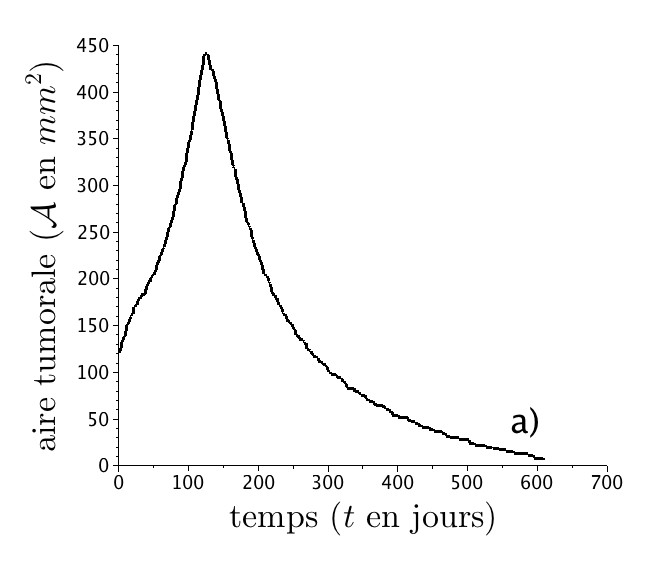
\includegraphics[width=0.31\textwidth]{possibilites/glivec_efficace.png}
}
\renewcommand{\thesubfigure}{b-c-d}
\subfloat[Imatinib à partir du jour 119 jusqu'au jour 867 puis sunitinib juste après ]{
\label{fig:possibilites2}
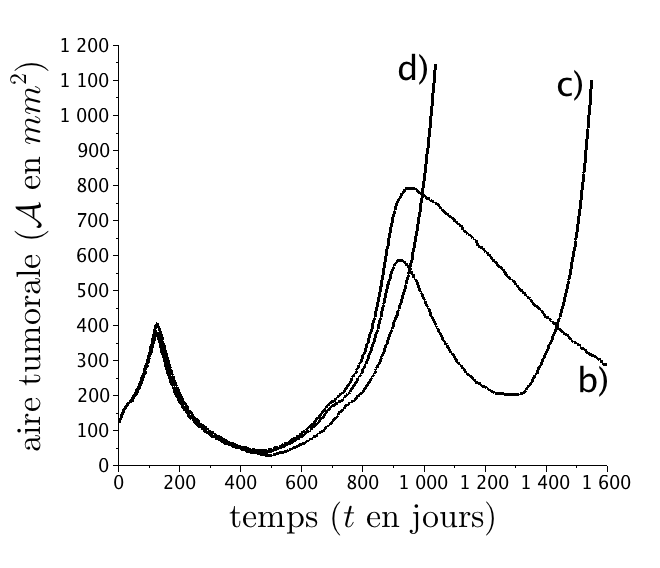
\includegraphics[width=0.31\textwidth]{possibilites/glivec_rechute.png}
}
\renewcommand{\thesubfigure}{e-f-g}
\subfloat[Imatinib à partir du jour 119 jusqu'au jour 300 puis sunitinib juste après ]{
\label{fig:possibilites3}
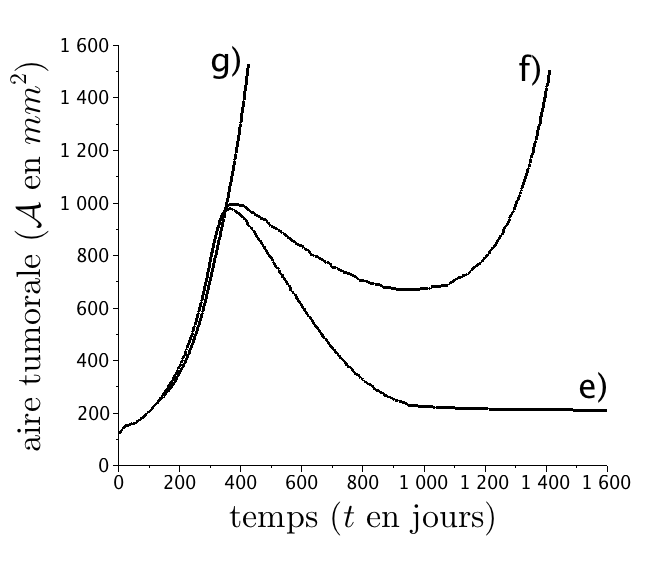
\includegraphics[width=0.31\textwidth]{possibilites/glivec_inefficace.png}
}
\caption{\label{fig:possibilites} 
Différents comportements pris en compte par notre modèle.
}
\end{figure}

Notre modèle reproduit les données cliniques pour \Nber et \Chen. De plus, il est capable de traiter l'ensemble des comportements rapportés par les médecins comme le montre la Figure~\ref{fig:possibilites} 
(\cf Table~\ref{table_param_possibilites} dans la section des informations complémentaires pour les differentes valeurs des paramètres utilisés):
\begin{enumerate}[label={\alph{*})}]
\item La métastase est contrôlée par le traitement~$\TI$ (imatinib). 
Dans ce cas, il n'y a pas besoin de changer de traitement. 
\item La métastase est contrôlée par le traitement~$\TI$ mais la tumeur recroît ensuite. Le traitement~$\TS$ (sunitinib ou sorafenib) est alors administré avec succès et l'aire tumorale est contrôlée. 
\item La métastase est contrôlée par le traitement~$\TI$ avant une première rechute. Le traitement~$\TS$ (sunitinib ou sorafenib) est alors administré et est efficace avant une seconde rechute. 
\item La métastase est contrôlée par le traitement~$\TI$ avant une première rechute. Ensuite le traitement~$\TS$ est totalement inefficace. 
\item Le traitement~$\TI$ est totalement inefficace. 
Ensuite le traitement~$\TS$ est efficace et l'aire de la tumeur est contrôlée. 
\item Le traitement~$\TI$ est totalement inefficace. 
Ensuite le traitement~$\TS$ est efficace avant une rechute.
\item Le traitement~$\TI$ est totalement inefficace. 
Ensuite le  traitement~$\TS$ est totalement inefficace. 
Ce type de profil est représentatif des patients avec une mutation génétique EXON, comme rapporté par Andersson
{\it et al.}~\cite{Andersson2006}, ou Hirota {\it et al.}~\cite{Hirota1998}.
\end{enumerate}



\FloatBarrier
\section{Conclusion}

Dans cet article, nous avons fourni un modèle dépendant de chaque patient, basé sur des EDPs, qui décrit le comportement global de métastases hépatiques de GISTs durant les différentes étapes. Nous avons présenté les méthodes numériques utilisées pour résoudre le système d'EDPs et nous avons introduit un nouveau type de schéma WENO5, appelé \twinweno. 
Ensuite, le modèle a été numériquement comparé avec les observations cliniques concernant \Nber, qui a été traité successivement à l'imatinib puis au sunitinib.
Comme présenté sur la 
Figure~\ref{fig:fit_area_henbert}, notre modèle fournit des résultats qui sont qualitativement en accord avec les données cliniques. En particulier, notre modèle est capable de décrire non seulement l'évolution de la taille de la lésion, mais aussi sa structure, comme l'illustrent les Figures~\ref{fig_nber} et~\ref{fig:compare_spatial_nber}.

Il est intéressant de noter que nos simulations numériques font apparaître une couronne de cellules proliférantes sur le pourtour de la tumeur juste avant la rechute. Ceci semble corroboré dans les scanners par l'augmentation de l'hétérogénéité tumorale, au sens des niveaux de gris, avant la rechute. Plus la métastase est hétérogène, plus la rechute est imminente. Ce résultat souligne le fait que le critère RECIST n'est pas suffisant pour évaluer l'efficacité d'un traitement.


Nous avons également étudié numériquement l'effet du paramètre~$\muI$, lié à l'efficacité du traitement~$\TI$. Nous avons montré que, selon notre modèle, augmenter la valeur de~$\muI$, ce qui peut être vu comme une augmentation de la dose administrée, ne fournit pas de meilleurs résultats en terme de survie sans aggravation comme le montre la Figure~\ref{fig:eff_glivec_nber}.


Il est important de noter que notre modèle fite bien les données, cependant il n'est pas prédictif. En effet, comme expliqué par la Figure~\ref{fig:possibilites2}, on peut voir que les 3 comportements typiques~$\rm{b,c,d}$ peuvent être obtenus avec le même comportement durant les 400 premiers jours. Ceci est dû au fait que sur les images médicales, il est compliqué de dire {\it à priori}, ce qu'il va se passer avant d'utiliser le second traitement, entre une tumeur principalement composée de la population~$P_2$ (comme pour le cas~${\rm b}$) de la Figure~\ref{fig:possibilites2}) ou une tumeur avec une population~$P_3$ (comme donné par la courbe~${\rm d}$) de la  Figure~\ref{fig:possibilites2}). En d'autre termes, on peut trouver différents jeux de paramètres qui donnent le même comportement initial. Ceci signifie que des données plus précises, comme de l'imagerie fonctionnelle, devront être nécessaires pour une meilleure analyse de la structure interne de la métastase. 


En conclusion, nous avons fourni un modèle qui fite avec les scanners cliniques que nous avons. De futurs travaux consisteront à ajouter plus d'informations biologiques que nous ne pouvons pas obtenir depuis les scanners, afin d'obtenir un modèle prédictif. L'imagerie fonctionnelle (TEP-scan ou IRM) ou des biopsies pourraient enrichir le présent modèle.


\section*{Remerciements}

Les données médicales utilisées dans cet article ont été fournies aux auteurs  par l'Institut Bergoni\'e, F-33000, Bordeaux, France. Nous remercions l'Institut Bergoni\'e pour sa collaboration et particulièrement l'oncologue MD Binh Bui.


Cette étude a été soutenue dans le cadre du LABEX TRAIL, ANR-10-LABX-0057 avec le soutien financier de l'Etat Francais, géré par l'Agence Nationale de Recherche (ANR) de France dans le cadre des "Investissements d'avenir" du Programme IdEx  (ANR-10-IDEX-03-02).

Les expérimentations présentées dans cet article ont été réalisées en utilisant la plateforme expérimentale PlaFRIM, développée par l'action de développement  Inria DIHPES avec le support du LABRI et de l'IMB et d'autres entités~: Conseil R\'egional d'Aquitaine, FeDER, Universit\'e de Bordeaux et CNRS (\textit{cf.} https://plafrim.bordeaux.inria.fr/)


Le Travail de Patricio Cumsille (PC) a été partiellement soutenu par le Programme de Recherche Associative (PIA) du Conicyt avec le financement numéro FB0001. Le travail de PC a aussi été partiellement soutenu par l'Université de B\'{\i}o-B\'{\i}o avec les financements DIUBB 121909 GI/C et DIUBB 122109 GI/EF.


Les auteurs remercient très chaleureusement Dr H. Fathallah-Shaykh pour ses discussions et ses conseils qui ont significativement contribués à l'amélioration de la qualité de cet article. 

%%-----------------------------
%%       bibliography
%%-----------------------------

\bibliographystyle{plain}
\bibliography{biblio}

\section{Informations complémentaires}

L'ensemble des paramètres utilisés pour réaliser la simulation numérique présentée Figure~\ref{fig:possibilites} de la section~\ref{section_possibilites} 
est présenté dans la Table~\ref{table_param_possibilites}.

\begin{table}[h]
\centering
\rowcolors{2}{gray!40}{white}
{\small
\begin{tabular}{|*{8}{p{15mm}|}}
\hline
\rowcolor[gray]{0.7} 
Nom & a) & b) & c) &d) &e) &f) &g) \\
\hline
\input{../data/params_value/table_possibilites.txt}
\hline \hline \hline
$L,D$ &6 &6 &6 &6 & 6 & 6 &6 \\
$N_x,N_y$ & 120 &120 & 120 &120 &120 &120&120\\
$r_1,r_2$ & 0.62& 0.62& 0.62& 0.62& 0.62& 0.62 & 0.62\\
$e$ & 0 &0&0&0&0&0&0\\
$\beta$ & 0 &0&0&0&0&0&0\\
\hline
\end{tabular}
}
\caption{\label{table_param_possibilites}Valeur des paramètres pour les courbes présentées Figure~\ref{fig:possibilites}.}
\end{table}
\FloatBarrier


\end{document}